\documentclass[preprint, 3p, authoryear]{elsarticle} %review=doublespace preprint=single 5p=2 column
%%% Begin My package additions %%%%%%%%%%%%%%%%%%%

\usepackage[hyphens]{url}

  \journal{Journal of Archaeological Sciences} % Sets Journal name

\usepackage{lineno} % add
  \linenumbers % turns line numbering on

\usepackage{graphicx}
%%%%%%%%%%%%%%%% end my additions to header

\usepackage[T1]{fontenc}
\usepackage{lmodern}
\usepackage{amssymb,amsmath}
\usepackage{ifxetex,ifluatex}
\usepackage{fixltx2e} % provides \textsubscript
% use upquote if available, for straight quotes in verbatim environments
\IfFileExists{upquote.sty}{\usepackage{upquote}}{}
\ifnum 0\ifxetex 1\fi\ifluatex 1\fi=0 % if pdftex
  \usepackage[utf8]{inputenc}
\else % if luatex or xelatex
  \usepackage{fontspec}
  \ifxetex
    \usepackage{xltxtra,xunicode}
  \fi
  \defaultfontfeatures{Mapping=tex-text,Scale=MatchLowercase}
  \newcommand{\euro}{€}
\fi
% use microtype if available
\IfFileExists{microtype.sty}{\usepackage{microtype}}{}

\ifxetex
  \usepackage[setpagesize=false, % page size defined by xetex
              unicode=false, % unicode breaks when used with xetex
              xetex]{hyperref}
\else
  \usepackage[unicode=true]{hyperref}
\fi
\hypersetup{breaklinks=true,
            bookmarks=true,
            pdfauthor={},
            pdftitle={Your horse is a donkey! Identifying domesticated equids from Western Iberia using collagen fingerprinting},
            colorlinks=false,
            urlcolor=blue,
            linkcolor=magenta,
            pdfborder={0 0 0}}

\setcounter{secnumdepth}{5}
% Pandoc toggle for numbering sections (defaults to be off)


% tightlist command for lists without linebreak
\providecommand{\tightlist}{%
  \setlength{\itemsep}{0pt}\setlength{\parskip}{0pt}}

% From pandoc table feature
\usepackage{longtable,booktabs,array}
\usepackage{calc} % for calculating minipage widths
% Correct order of tables after \paragraph or \subparagraph
\usepackage{etoolbox}
\makeatletter
\patchcmd\longtable{\par}{\if@noskipsec\mbox{}\fi\par}{}{}
\makeatother
% Allow footnotes in longtable head/foot
\IfFileExists{footnotehyper.sty}{\usepackage{footnotehyper}}{\usepackage{footnote}}
\makesavenoteenv{longtable}

% Pandoc citation processing
\newlength{\cslhangindent}
\setlength{\cslhangindent}{1.5em}
\newlength{\csllabelwidth}
\setlength{\csllabelwidth}{3em}
\newlength{\cslentryspacingunit} % times entry-spacing
\setlength{\cslentryspacingunit}{\parskip}
% for Pandoc 2.8 to 2.10.1
\newenvironment{cslreferences}%
  {}%
  {\par}
% For Pandoc 2.11+
\newenvironment{CSLReferences}[2] % #1 hanging-ident, #2 entry spacing
 {% don't indent paragraphs
  \setlength{\parindent}{0pt}
  % turn on hanging indent if param 1 is 1
  \ifodd #1
  \let\oldpar\par
  \def\par{\hangindent=\cslhangindent\oldpar}
  \fi
  % set entry spacing
  \setlength{\parskip}{#2\cslentryspacingunit}
 }%
 {}
\usepackage{calc}
\newcommand{\CSLBlock}[1]{#1\hfill\break}
\newcommand{\CSLLeftMargin}[1]{\parbox[t]{\csllabelwidth}{#1}}
\newcommand{\CSLRightInline}[1]{\parbox[t]{\linewidth - \csllabelwidth}{#1}\break}
\newcommand{\CSLIndent}[1]{\hspace{\cslhangindent}#1}

\usepackage{wasysym}
\sloppy
\usepackage{subfig}
\usepackage{booktabs}
\usepackage{longtable}
\usepackage{array}
\usepackage{multirow}
\usepackage{wrapfig}
\usepackage{float}
\usepackage{colortbl}
\usepackage{pdflscape}
\usepackage{tabu}
\usepackage{threeparttable}
\usepackage{threeparttablex}
\usepackage[normalem]{ulem}
\usepackage{makecell}
\usepackage{xcolor}



\begin{document}


\begin{frontmatter}

  \title{Your horse is a donkey! Identifying domesticated equids from Western Iberia using collagen fingerprinting}
    \author[Universidade de Évora,Laboratório HERCULES,Sapienza Università di Roma]{Roshan Paladugu%
  \corref{cor1}%
  \fnref{1}}
   \ead{rpaladugu@uevora.pt} 
    \author[Harvard University]{Kristine Korzow-Richter%
  %
  \fnref{1}}
   \ead{krichter@fas.harvard.edu} 
    \author[Universidade do Algarve]{Maria João Valente%
  %
  \fnref{2}}
   \ead{mvalente.ualg@fastmail.com} 
    \author[Laboratório de Arqueociências (DGPC),Universidade do Porto,Universidade de Lisboa]{Sónia Gabriel%
  %
  \fnref{2}}
   \ead{gabriel.sonia@gmail.com} 
    \author[Universidade de Lisboa]{Cleia Detry%
  %
  \fnref{2}}
   \ead{cleiadetry@campus.ul.pt} 
    \author[Harvard University,Max Planck Institute for Evolutionary Anthropology]{Christina Warinner%
  %
  \fnref{2}}
   \ead{warinner@fas.harvard.edu} 
    \author[Universidade de Évora,Laboratório HERCULES]{Cristina Barrocas Dias%
  %
  \fnref{2}}
   \ead{cmbd@uevora.pt} 
      \affiliation[Universidade de Évora]{Departamento de Química, Escola de Ciências e Tecnologia, Colégio Luís António Verney, Rua Romão Ramalho 59, Évora, Portugal (7000-671)}
    \affiliation[Universidade de Lisboa]{Uniarq-Centro de Arqueologia da Universidade de Lisboa, Faculdade de Letras da Universidade de Lisboa, Alameda da Universidade, Lisboa, Portugal (1600-214)}
    \affiliation[Laboratório HERCULES]{Laboratório HERCULES, Universidade de Évora, Palácio do Vimioso, Largo Marquês de Marialva 8, Évora, Portugal (7000-554)}
    \affiliation[Sapienza Università di Roma]{Dipartimento di Biologia Ambientale, Sapienza Università di Roma, Piazzale A. Moro 5, 00185 Roma, Italy}
    \affiliation[Harvard University]{Peabody Museum 570, 11 Divinity Ave, Cambridge, MA 02138, United States of America}
    \affiliation[Universidade do Porto]{CIBIO - InBIO, Campus de Vairão, R. Monte de Vairão, Vila do Conde, Portugal (4485-167)}
    \affiliation[Laboratório de Arqueociências (DGPC)]{Calçada do Mirante à Ajuda 10A, Lisboa, Portugal (1300-418)}
    \affiliation[Max Planck Institute for Evolutionary Anthropology]{Deutscher Platz 6, Leipzig, Germany (04103)}
    \cortext[cor1]{Corresponding author}
    \fntext[1]{Corresponding Author}
    \fntext[2]{Equal contribution}
  
  \begin{abstract}
  Skeletal remains of two equid species, \emph{Equus caballus} (horse) and \emph{Equus asinus} (donkey), have been found in archaeological contexts throughout Iberia since the Paleolithic and Chalcolithic periods, respectively. These two species play different economic and cultural roles, and therefore it is important to be able to distinguish between the two species to better understand their relative importance in the past human societies. The most reliable morphological features for distinguishing between the two domesticated equids are based on cranial measurements and tooth enamel folds, leading to only a small percentage of archaeological remains that can be identified to species. Ancient DNA (aDNA) analysis can be used to reliably distinguish the two \textcolor{blue}{equids}, but it can be cost prohibitive to apply to large assemblages, and aDNA preservation of non-cranial elements is often low. Collagen peptide mass fingerprinting by matrix-assisted laser desorption time-of-flight (MALDI-TOF) mass spectrometry, also known as zooarchaeology by mass spectrometry (ZooMS), is a minimally destructive and cost-effective alternative to aDNA analysis for taxonomic determination. However, current ZooMS markers lack resolution below the genus level \emph{Equus}. In this paper, we report a novel ZooMS peptide marker that reliably distinguishes between horses and donkeys using the enzyme chymotrypsin. We apply this peptide marker to taxonomically identify bones from the Iberian Peninsula ranging from the Iron Age to the Late Modern Period. The peptide biomarker has the potential to facilitate the collection of morphological data for zooarchaeological studies of equids in Iberia and throughout Eurasia and Africa.
  \end{abstract}
    \begin{keyword}
    Peptide mass fingerprinting \sep Zooarchaeology \sep Bone \sep Palaeontology \sep Archaeology \sep 
    ZooMS
  \end{keyword}
  
 \end{frontmatter}

\hypertarget{introduction}{%
\section{Introduction}\label{introduction}}

Horse (\emph{Equus caballus} / \emph{Equus ferus}) and donkey (\emph{Equus asinus}) along with their hybrids are important large domesticates in Holocene archaeological contexts. Domestic equids have played roles in the economy, travel, and conflicts of past societies. Horses have been utilised for riding, racing, and as mounts in war due to their intelligence and speed (Clutton-Brock, 1992; Hanot and Bochaton, 2018). Donkeys, on the other hand, have been appreciated for their endurance and adaptations to harsh environments, leading them to be utilised for load-bearing (Baxter, 1998; Kimura et al., 2013). Accurate identification of domestic equids and their hybrids is an arduous but imperative task in archaeological studies. With the exception of situations where one of the species is entirely absent, it is usually difficult to distinguish between horse and donkey remains based on skeletal \textcolor{blue}{morphological} criteria alone (Hanot and Bochaton, 2018).

Conventional criteria for zooarchaeological identification are based on the morphology of teeth enamel folds (Armitage and Chapman, 1979; Davis, 1980; Eisenmann, 1986, 1981, 1980; Uerpmann, 2002), the skull (Albizuri and Nadal, 1991; Azzaroli, 1978; Eisenmann, 1986, 1980; Groves and Mazák, 1967; Kunst, 2000), and \textcolor{blue}{a few} post-cranial elements (Arloing, 1882; Eisenmann and Beckouche, 1986; Hanot and Bochaton, 2018; Peters, 1998). One problem with many of these criteria is that they are dependent on bone size and assume that horses and hybrids are larger than donkeys (Forest, 2008; Hanot et al., 2017), which is not always accurate even when entire skeletons are available for analysis. More practically, intact skulls with complete post-cranial remains are rarely encountered in the archaeological record, and equids are more often represented by individual or fragmented bones that are difficult to taxonomically assign based on size. For example, two recent studies from England and Poland point out that horse bones at archaeological sites are partially the result of distinctive depositional processes, including the standardised post-mortem processing of their carcasses away from domestic sites at tanneries and knackers' yards (Ameen et al., 2021; Jaworski et al., 2020). Species level determinations are most frequently made using teeth (Chuang and Bonhomme, 2019; Davis, 1980; Eisenmann, 1986, 1981, 1980), which generally represent a relatively small proportion of faunal assemblages. Further complicating species level identifications is the fact that equids are less frequently consumed than other domesticates, such as cattle, caprines, and suids. This leads to fewer measurable bones recovered from some sites, and consequently less morphological data is available to determine site-specific size profiles (Hanot and Bochaton, 2018).

The most reliable means of taxonomic identification of archaeological equids has been through ancient DNA (aDNA) analyses (Cucchi et al., 2017; Jónsson et al., 2014; Vilstrup et al., 2013; Weinstock et al., 2005), which comes with its own challenges, especially in regions such as the Iberian Peninsula that have very low success rates (10\% -- 30\%). Ancient DNA analyses can also be costly, especially when analysing large assemblages. \textcolor{blue}{Proteins, especially collagen, can be used to overcome these limitations. The most affordable and high-throughput option is zooarchaeology by mass spectrometry (ZooMS) which utilizes differences in collagen type I (COL1) sequences to distinguish between taxonomic groups. While there are variations in the collagen sequence between horse and donkey, previously published ZooMS markers provide taxonomic resolution only to the genus level in equids, thereby limiting the usefulness of this technique for studying species of \emph{Equus}} (Buckley et al., 2017, 2009; Buckley and Collins, 2011; Kirby et al., 2013; Welker et al., 2016). \textcolor{blue}{Tandem mass spectrometry (LC-MS/MS) based methods, including SPIN, can reliably distinguish between horse and donkey using the differences in COL1} (Rüther et al., 2022), \textcolor{blue}{but even targeted LC-MS/MS based analyses are still more expensive and require more computational power than ZooMS. ZooMS therefore remains the most cost-effective biomolecular method for rapid and high-throughput taxonomic identification. As such ZooMS is highly suited to the analysis of large faunal assemblages, is ideal for projects with limited budgets, and can be productively used to pre-screen samples for preservation prior to more expensive methods, such as aDNA or LC-MS/MS analyses.} In this manuscript we successfully utilised \textcolor{blue}{a new ZooMS} peptide marker to successfully distinguish horses and donkeys from Western Iberian Holocene contexts.

\hypertarget{domesticated-equids-in-iberia}{%
\section{Domesticated equids in Iberia}\label{domesticated-equids-in-iberia}}

Both horse and donkey were domesticated in different regions almost concurrently around 5000 - 4200 years ago, with the horse being domesticated in Western Eurasian steppes (Librado et al., 2021; Warmuth et al., 2012) and the donkey in Northern Africa (Beja-Pereira et al., 2004; Rossel et al., 2008; Todd et al., 2022).

Iberian Peninsula has been home to wild or domesticated horses since the Holocene (Warmuth et al., 2012). Equid bones have been reported continuously in the Western part of Iberia from the Late Pleistocene through the Medieval Period until the Modern Period (Cardoso, 1995, 1994, 1993; Davis et al., 2008; Davis, 2006; Detry et al., 2016; Detry, 2007; Detry and Arruda, 2013; Detry and Fabião, 2021; Morales Muñiz et al., 1998; Rowley-Conwy, 1993; Valente, 2008). During the Early and Middle Neolithic equid bones have only been reported from the site of Lameiras in Portugal (Valente and Carvalho, 2019, 2014). By \textcolor{blue}{the} Late Neolithic, equid remains become more abundant but still scarce in comparison to other species. The notable exception is the Late Neolithic site of Xacafre (Portugal) where more than 100 equid remains have been recovered (Aleixo, 2018). With the advent of the Chalcolithic and Bronze Ages, there is an increase in the number of equid remains across sites in the Iberian Peninsula (Castaños, 2005; Harrison et al., 1987; Morales Muñiz et al., 1998).

The extinct Iberian wild ass (\emph{Equus hydruntinus}) has been found in Middle Palaeolithic, Neolithic, and Chalcolithic contexts from Portugal and Spain. Although some populations might have remained in Iberia until first millennium BCE (Schuhmacher et al., 2009), there is no evidence of domestication (Cardoso and Detry, 2002; Davis, 2002; Davis et al., 2018). It is widely accepted that domestic donkeys from North Africa were introduced to the Iberian Peninsula by the Phoenicians as early as the 8\textsuperscript{th} century BCE (von den Driesch and Boessneck, 1985). However, earlier dates have been proposed based on the discovery of a molar tooth, confirmed by mitochondrial DNA analysis to be donkey, at the Chalcolithic site of Leceia (Cardoso et al., 2013). This is not surprising given that artefacts of North African origin, such as ivory and ostrich eggshells, have been reported in Portugal and South-West Spain from the Late Neolithic/Chalcolithic onwards (Schuhmacher et al., 2009; Valera et al., 2015; Valério et al., 2018). Skeletal elements of donkey are found in higher numbers starting in the Iron Age, with a noticeable increase during the Roman \textcolor{blue}{Period} and Middle Ages (Davis et al., 2008; Davis, 2006; Davis and Gonçalves, 2017; Detry et al., 2016; Detry and Arruda, 2013; Detry and Pimenta, 2017). In this complex scenario with significant archaeological questions regarding the presence and use of domesticated equids, ZooMS would be a valuable, cost-effective, and reliable tool to (1) increase identification rate of horse and donkey remains across time periods \textcolor{blue}{and} (2) interpret slaughter and birthing patterns similar to other domesticates (Castaños, 2005).

\hypertarget{zooms-markers-for-equids}{%
\section{ZooMS markers for equids}\label{zooms-markers-for-equids}}

ZooMS is a peptide mass fingerprinting technique developed to assign taxonomic identities based on COL1 peptide masses. The primary principle of ZooMS is to generate a peptide mass fingerprint from tryptic digests of bone or other collagen containing tissues using a matrix-assisted laser desorption/ionization time-of-flight (MALDI-TOF) mass spectrometer. In the past decade, researchers have successfully leveraged this technique to distinguish the genus \emph{Equus} from other large mammal taxa in archaeological records using a standard panel of nine peptide markers (Buckley et al., 2017, 2009; Buckley and Collins, 2011; Kirby et al., 2013; Welker et al., 2016). However, these markers are invariant across all published species in the \emph{Equus} genus (Table S1), which makes them unsuitable for species level identification. Recent studies have developed alternative markers for other regions of the collagen protein where amino acid differences allow for better taxonomic resolution of specific taxonomic groups, such as marsupials and bovids (Coutu et al., 2021; Janzen et al., 2021; Peters et al., 2021). Here we use genetic data to identify collagen sequence differences between horses and donkeys and confirm a species specific ZooMS marker using a chymotrypsin digestion that can reliably distinguish horses from donkeys across a range of archaeological sites.

\begin{table}[H]

\caption{\label{tab:eqtable1}Overview of archaeological and taxonomic reference samples.}
\centering
\begin{tabular}[t]{cccc}
\toprule
Sample Type & Time Period & Country & Number of samples (n)\\
\midrule
 & Iron Age & Spain & 5\\
\cmidrule{2-4}
 & Roman & Portugal & 23\\
\cmidrule{2-4}
 & Late Antiquity & Portugal & 3\\
\cmidrule{2-4}
 & Medieval & Portugal & 5\\
\cmidrule{2-4}
 & Medieval & Spain & 3\\
\cmidrule{2-4}
\multirow{-6}{*}{\centering\arraybackslash Archaeological} & Late Modern & Portugal & 1\\
\cmidrule{1-4}
Taxonomic Reference & Modern & Portugal & 6\\
\bottomrule
\end{tabular}
\end{table}

\hypertarget{material-and-methods}{%
\section{Material and methods}\label{material-and-methods}}

\hypertarget{samples}{%
\subsection{Samples}\label{samples}}

Reference bone samples (Table \ref{tab:eqtable1}) of horse and donkey (3 of each species) were sourced from the Mammalogy collection of Laboratório de Arqueociências (Direção Geral do Património Cultural, Lisbon). 20 -- 30 mg bone samples were taken from non-diagnostic sections of the bones. Archaeological samples (n = 40) originate from various sites across Portugal and Spain (Table \ref{tab:eqtable1}) ranging from the Early Iron Age to Early Modern period. Some of the samples were identifiable by morphology as either horse or donkey (n = 15) while the majority were only identifiable to the genus \emph{Equus} (n = 25). From each archaeological bone a 10-40 mg sample was clipped (bone fragment) or drilled (bone powder) from a non-diagnostic portion of the bone.

\hypertarget{collagen-extraction}{%
\subsection{Collagen extraction}\label{collagen-extraction}}

Collagen was extracted from both the reference and archaeological samples based on previously published acid-insoluble (Buckley et al., 2009; Welker et al., 2015) and acid-soluble (Brown et al., 2022; van der Sluis et al., 2014) protocols. Three blanks were extracted after every 12 samples as controls. All samples were first extracted using the acid-insoluble method. If this method failed due to either the samples degrading entirely in acid or if poor spectra were produced, the acid-\textcolor{blue}{soluble} method was used. Briefly bone fragments or powder were demineralised in 500 \(\mu\)l of 0.6M \textcolor{blue}{hydrochloric acid} (\emph{HCl}) for 48 hours after which the supernatant was collected and stored for \textcolor{blue}{the} acid-\textcolor{blue}{soluble} method. The samples were rinsed 3 times with 200 \(\mu\)l of 50 mM ammonium bicarbonate \textcolor{blue}{\emph{$NH_{4}HCO_{3}$}}, \textcolor{blue}{pH 8} (AmBic), followed by an incubation for 5 minutes at room temperature in 200 \(\mu\)l of of 0.1M \textcolor{blue}{sodium hydroxide} (\emph{NaOH}) to remove fulvic and humic acids. The samples were then rinsed three times with AmBic. 100 \(\mu\)l of AmBic was added to the samples and they were gelatinized by incubating for 1 hour at 65 \(\text{\textdegree}\)C.

For the acid-soluble method the acid supernatant was filtered using a 30 kDa ultrafilter and centrifugation (3700 rpm). The samples were washed twice by adding 500 \(\mu\)l of AmBic to the ultrafilter and centrifuged. 100 \(\mu\)l of AmBic was added to the top of the filter and the collagen was resuspended through pipetting. The AmBic was then removed from the filter into a clean centrifuge tube.

\hypertarget{enzymatic-testing}{%
\subsection{Enzymatic testing}\label{enzymatic-testing}}

\textcolor{blue}{COL1} sequences from horse (XP\_023508478.1, XP\_008516208.1, XP\_001492989.1) and donkey (XP\_014689063.1, ACM24774.1, XP\_014708845.1, ACM24775.1) were aligned and analysed using Geneious\(^\text{\texttrademark}\) (R11.1) (Kearse et al., 2012). The sequences were theoretically digested with all of the enzymes available using PeptideMass\(^\text{\texttrademark}\) from Expasy\(^\text{\textregistered}\) (Gasteiger et al., 2005; Wilkins et al., 1997). The peptides containing the amino acid differences were then identified and enzymes where at least two of the differences were on peptides that would be visible within the mass range of the MALDI. In order to assess the actual viability of the enzymes the six reference samples, plus two well identified archaeological horse samples were analysed. Multiple gelatinisations were performed from the same digested bone and pooled to make 400 \(\mu\)l of extracted collagen. Then digestions were performed on 50 \(\mu\)l of extracted collagen for each digestion.

\emph{Tryptic digestions:} Digestions were performed in AmBic with 0.4 \(\mu\)g trypsin (Promega\(^\text{\textregistered}\) V5111) at 37 \(\text{\textdegree}\)C for 16-18 hours.

\emph{Glu-C digestions:} Extracted collagen was dried down and resuspended in 50 \(\mu\)l of 100 mM potassium phosphate buffer pH 8 and incubated with 0.8 \(\mu\)g Glu-C (Promega\(^\text{\textregistered}\) V1651) at 37 \(\text{\textdegree}\)C for 16-18 hours.

\emph{Thermolysin digestions:} Extracted collagen was dried down and resuspended in 50 \(\mu\)l of 50 mM Tris(hydroxymethyl)aminomethane hydrochloride, 0.5 mM calcium chloride, pH 8 and incubated with 0.8 \(\mu\)g thermolysin (Promega\(^\text{\textregistered}\) V4001) at 70 \(\text{\textdegree}\)C for 4 hours.

\emph{Chymotryptic digestions:} Extracted collagen was dried down and resuspended in 50 \(\mu\)l of Tris buffer (100 mM Tris(hydroxymethyl)aminomethane hydrochloride, 10 mM calcium chloride, pH 8.0) and incubated with 0.4 \(\mu\)g chymotrypsin (Promega \(^\text{\textregistered}\) V1061) at 25 \(\text{\textdegree}\)C for 16 -- 18 hours.

Dual digestion was performed with trypsin and chymotrypsin. Extracted collagen was dried down and resuspended in 50 \(\mu\)l of Tris buffer. One set of samples were digested with 0.4 \(\mu\)g of trypsin and 0.8 \(\mu\)g of chymotrypsin at 25 \(\text{\textdegree}\)C for 16 -- 18 hours. A second set of samples were digested with 0.8 \(\mu\)g of chymotrypsin at 25 \(\text{\textdegree}\)C for 16 -- 18 hours. Then 0.4 \(\mu\)g of trypsin was added and the samples were incubated at 37 \(\text{\textdegree}\)C for 30 minutes. All digestions were stopped by adding 1 \(\mu\)l of 5\% trifluoroacetic acid (TFA).

\hypertarget{archaeological-digestions}{%
\subsection{Archaeological digestions}\label{archaeological-digestions}}

Subsequent archaeological samples were gelatinized once and the resulting 100 \(\mu\)l of extracted collagen was split in half and digested separately with trypsin and chymotrypsin as described above.

\hypertarget{peptide-mass-fingerprinting-and-data-analysis}{%
\subsection{Peptide mass fingerprinting and data analysis}\label{peptide-mass-fingerprinting-and-data-analysis}}

All digests were spotted in both undiluted and diluted 1:10 \textcolor{blue}{in 50\% acetonitrile (ACN), 0.1\% TFA}, in duplicate on a BRUKER\(^\text{\textregistered}\) MTP Groundsteel\(^\text{\texttrademark}\) 394-target plate with equal volume of matrix (10 mg of \(\alpha\)-cyano-4-hydroxycinnamic acid in 1 ml of 50\% ACN/0.1\% TFA).

Samples were analysed on a Bruker\(^\text{\textregistered}\) Ultraflextreme\(^\text{\texttrademark}\) MALDI-TOF/TOF (Bruker Daltonics\(^\text{\textregistered}\)) with a smartbeam-II laser. A SNAP averaging algorithm was used to obtain monoisotopic masses (C: 4.9384, N: 1.3577, O: 1.4773, S: 0.0417, H: 7.7583) at the Harvard Center for Mass Spectrometry.

The resulting spectra were analysed using mMass (Strohalm et al., 2010). Spectra were assessed for presence of predicted or confirmed marker peaks based upon a S/N ratio of at least 3. Identification of tryptic ZooMS spectra was done based upon published markers (Buckley et al., 2017, 2009; Buckley and Collins, 2011; Kirby et al., 2013; Welker et al., 2016). The best spectrum \textcolor{blue}{from trypsin and chymotrypsin digestions} for each sample is available at Zenodo (\href{https://doi.org/doi:10.5281/zenodo.6878868}{10.5281/zenodo.6878868}).

\hypertarget{marker-identification-and-confirmation}{%
\subsection{Marker identification and confirmation}\label{marker-identification-and-confirmation}}

After analysis of the MALDI data, one sample from each species was analysed using LC-MS/MS at the Harvard Center for Mass Spectrometry. 4 \(\mu l\) of chymotryptic digested collagen was analysed on an Orbitrap\(^\text{\texttrademark}\) Elite mass spectrometer (Thermo Scientific\(^\text{\textregistered}\)) coupled with an Waters nanoACQUITY\(^\text{\texttrademark}\) HPLC pump (Waters\(^\text{\textregistered}\) AG). Peptides were separated onto a 100-\(\mu m\) inner diameter microcapillary trapping column packed first with approximately 5 cm of C18 ReproSil\(^\text{\texttrademark}\) resin (5 \(\mu m\), 100 Å, Dr.~Maisch\(^\text{\textregistered}\), Germany) followed by an analytical column \(\sim 20\) cm of ReproSil\(^\text{\texttrademark}\) resin (1.9 \(\mu m\), 200 Å, Dr.~Maisch\(^\text{\textregistered}\)). Separation was achieved by applying a gradient from 5\% to 27\% acetonitrile in 0.1\% formic acid over 90 minutes at 200 nl \(min ^{-1}\). Electrospray ionization was enabled by applying a voltage of 1.8 kV using a home-made electrode junction at the end of the microcapillary column and sprayed from fused silica pico tips (New Objective\(^\text{\texttrademark}\)). The LTQ Orbitrap\(^\text{\texttrademark}\) Elite was operated in the data-dependent mode for the mass spectrometry methods. The mass spectrometry survey scan was performed in the Orbitrap\(^\text{\texttrademark}\) in the range of 400--1,800 m/z at a resolution of 6 × 104, followed by the selection of the 20 most intense ions (TOP20) for collision-induced dissociation (CID)-tandem mass spectrometry fragmentation in the ion trap using a precursor isolation width window of 2 m/z, automatic gain control (AGC) setting of 10,000, and a maximum ion accumulation of 200 ms. Singly charged ion species were not subjected to CID fragmentation. Normalized collision energy was set to 35 V and an activation time of 10 ms, AGC was set to 50,000, and the maximum ion time was 200 ms. Ions in a 10-ppm m/z window around ions selected for tandem mass spectrometry were excluded from further selection for fragmentation for 60 seconds.

Resulting data was processed using Byonic\(^\text{\texttrademark}\) (v3.5.3) (74) in two steps. All runs had the following parameters: precursor mass tolerance: 10 ppm; fragment mass tolerance: 0.5 Da; Cleavage sites: C-terminal to tryptophan, phenylalanine, tyrosine, lysine, methionine, and histidine; with decoys. The first step was to identify any additional proteins in the sample other than collagen.

This was done using a database composed of Swissprot\(^\text{\texttrademark}\) (downloaded 13 May 2022) and the proteomes from horse (UP000002281, 44,487 proteins) and donkey (UP000694387, 33,257 proteins) and the parameters: fully specific cleavage, 2 missed cleaves, common modifications: deamidation on arginine and glutamine, oxidation of proline, methionine, and lysine; rare modifications: Glx to pyro-Glu on N-terminal glutamine and glutamic acid, ammonia loss on N-terminal cysteine; modifications allowed: common - 2, rare - 1. The peptide FDR rate cut off was 2\% and a focused database was made from the proteins identified. The focused databases were then combined and duplicates were removed. Col1 sequences were also removed and replaced with the six curated equid sequences (see above). \textcolor{blue}{In the second step}, this database was then used to identify the collagen peptide sequences using Byonic\(^\text{\texttrademark}\) with the following parameters: semi-specific cleavage, 2 missed cleaves, common modifications: deamidation on arginine and glutamine, oxidation of proline, methionine, and lysine; rare modifications: Glx to pyro-glu on N-terminal Q/E, ammonia loss on N-terminal C; modifications allowed: common - 6, rare - 1. The peptide FDR rate cut off was 1\%. \textcolor{blue}{For quality assurance these same parameters were also used with non-specific cleavage.}

\hypertarget{data-availability}{%
\subsection{Data availability}\label{data-availability}}

MALDI-TOF-MS spectra data have been deposited in Zenodo (https://doi.org/doi:10.5281/zenodo.6878868) and the LC-MS/MS spectra data have been deposited in ProteomeXchange (PXD035509) through Massive (MASSIVE MSV000089943) at https://doi.org/doi:10.25345/C5T727K8H. The R code and data used for the study can be accessed at \url{https://osf.io/qsc25/} for reproducibility and transparency. The code, data, and figures are licensed under CC BY 4.0 \url{http://creativecommons.org/licenses/by/4.0/}, to enable maximum re-use. \textcolor{blue}{All other data are included in the manuscript and/or supporting information.}

\hypertarget{results-and-discussion}{%
\section{Results and Discussion}\label{results-and-discussion}}

\hypertarget{identification-and-confirmation-of-biomarkers}{%
\subsection{Identification and confirmation of biomarkers}\label{identification-and-confirmation-of-biomarkers}}



\begin{figure*}
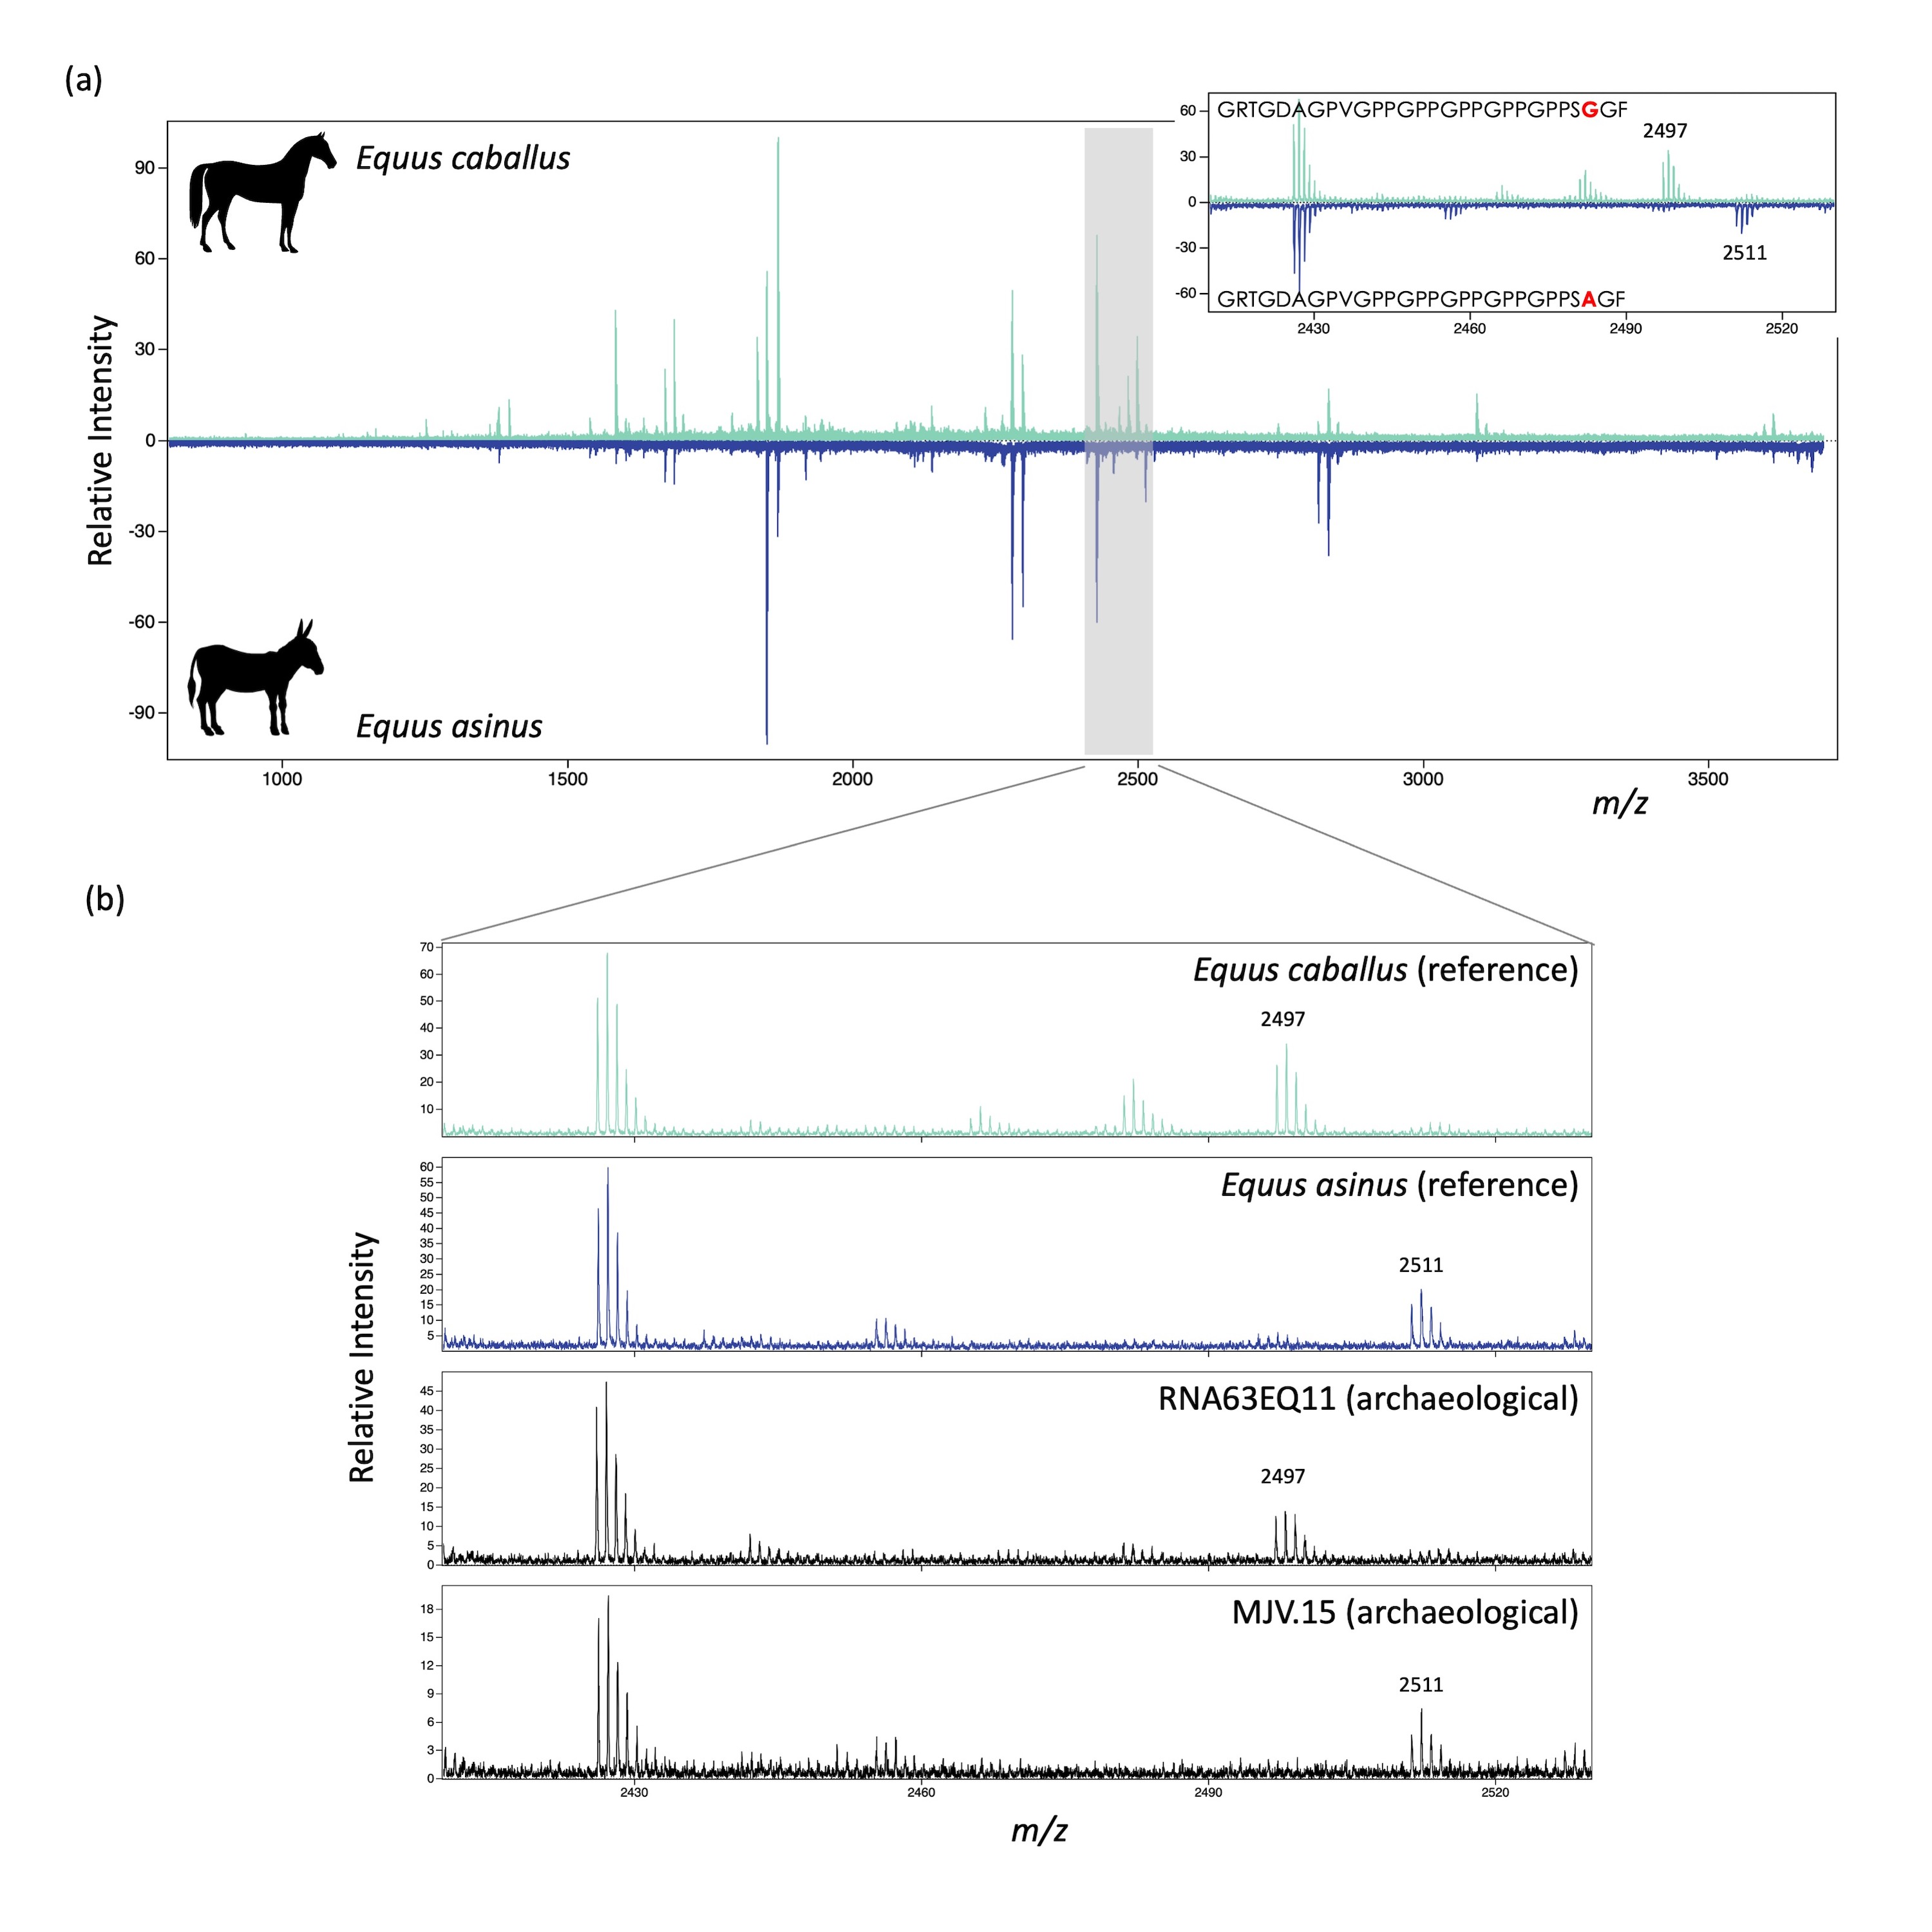
\includegraphics[width=1\linewidth]{../img/equid_marker} \caption{\textcolor{blue}{(a) MALDI spectra of chymotryptic peptides of COL1 for horse (light blue, top) and donkey (dark blue, bottom). The majority of the peaks present in the spectra are identical , with the major difference between the two spectra being the diagnostic marker with horse at m/z 2497 and donkey at m/z 2511 (inset). The sequence of the peptide confirmed by LC-MS/MS is shown with the single amino acid difference between the two species highlighted in red (inset). (b) The diagnostic portion of the MALDI spectra of the reference horse (light blue) and donkey (dark blue), as well as two archaeological samples identified as horse (RNA63EQ11) and donkey (MJV.15).}}\label{fig:equidmarkerplot}
\end{figure*}



\begin{table*}

\caption{\label{tab:eqtable2}Amino acid differences between horse and donkey COL1 proteins and their predicted visibility by MALDI following enzymatic digestion. Published COL1 sequence data were obtained from horse (XP\_023508478.1, XP\_008516208.1, XP\_001492989.1) and donkey (XP\_014689063.1, ACM24774.1, XP\_014708845.1, ACM24775.1). Proteins were digested in silico using Peptide Mass (Gattiker et al., 2002; Wilkins et al., 1997), and peptides were marked as theoretically visible if between \emph{m/z} 800 and \emph{m/z} 3500. Nomenclature of the amino acid locations after Brown et al. (2021a).}
\centering
\begin{tabular}[t]{cccccc}
\toprule
  & COL1A1 1016 & COL1A2 93 & COL1A2 336 & COL1A2 411 & COL1A2 887\\
\midrule
Horse & G & N & S & S & H\\
Donkey & A & K & T & T & N\\
Mass difference (Da) & 14 & 14 & 14 & 14 & 23\\
\addlinespace[1em]
\multicolumn{6}{l}{\textbf{Predicted visibility by MALDI-TOF following enzymatic digestion}}\\
\hspace{1em}Trypsin & -- & X$^{*}$ & -- & X & --\\
\hspace{1em}Glu-C$^{a}$ & X & X & X & -- & --\\
\hspace{1em}Chymotrypsin & -- & X & X & -- & --\\
\hspace{1em}Thermolysin & X & -- & -- & X & X\\
\bottomrule
\multicolumn{6}{l}{\rule{0pt}{1em}\textsuperscript{a} phosphate buffer.}\\
\multicolumn{6}{l}{\rule{0pt}{1em}\textsuperscript{*} visible in horse only as the amino acid difference is at a tryptic cut site.}\\
\end{tabular}
\end{table*}

Analysis of published collagen sequence data identified five amino acid differences between horse and donkey, one on the gene \emph{COL1A1} and four on \emph{COL1A2} (Table \ref{tab:eqtable2}). This is consistent with the known higher mutation rate of \emph{COL1A2}. Four enzymes (trypsin, Glu-C in a phosphate buffer, chymotrypsin, and thermolysin) cut at sites that should generate two or more peptides containing these amino acid differences based on in silico predictions. However, the MALDI spectra showed no peaks corresponding to these predicted peptides for any of the enzymes. Further analysis showed no consistent differences among \emph{Equus} species based on the MALDI spectra for trypsin, Glu-C, and thermolysin. This is not surprising as only part of the collagen protein is reliably visible in the MALDI spectra (Buckley et al., 2009; Janzen et al., 2021).

Spectra produced from the enzyme chymotrypsin had one consistently visible difference between the species corresponding to a 14 Da mass difference (Figure \ref{fig:equidmarkerplot}). However, the masses (\emph{m/z} 2497 and \emph{m/z} 2511) did not correspond to any of the masses of the theoretically chymotryptic digested peptides (Table \ref{tab:eqtable2}).

In order to assess the reliability and authenticity of this proposed marker we: (1) conducted LC-MS/MS analysis to sequence the peptide, and (2) compared the sequence data to enzyme activity profiles for chymotrypsin. LC-MS/MS confirmed the sequence of the candidate markers that covered the known amino acid difference between the species at COL1A1 1016 (horse: GRTGDAGPVGPPGPPGPPGPPGPPS\textbf{G}GF, donkey: GRTGDAGPVGPPGPPGPPGPPGPPS\textbf{A}GF) (SI Figure-1). However, the peptides were only cleaved on one end at a common chymotryptic cut site (C-terminal to phenylalanine) and the other site is not commonly reported as a chymotryptic cut site (C-terminal to \textcolor{blue}{arginine before} the glycine in the reported peptide). Because trypsin cuts C-terminal to an arginine, dual digestions with chymotrypsin and trypsin were attempted. However due to the differences in activity between trypsin and chymotrypsin, only the fully tryptic peaks were visible in the MALDI-TOF spectra \textcolor{blue}{for} both dual and sequential digestions.



\begin{figure*}
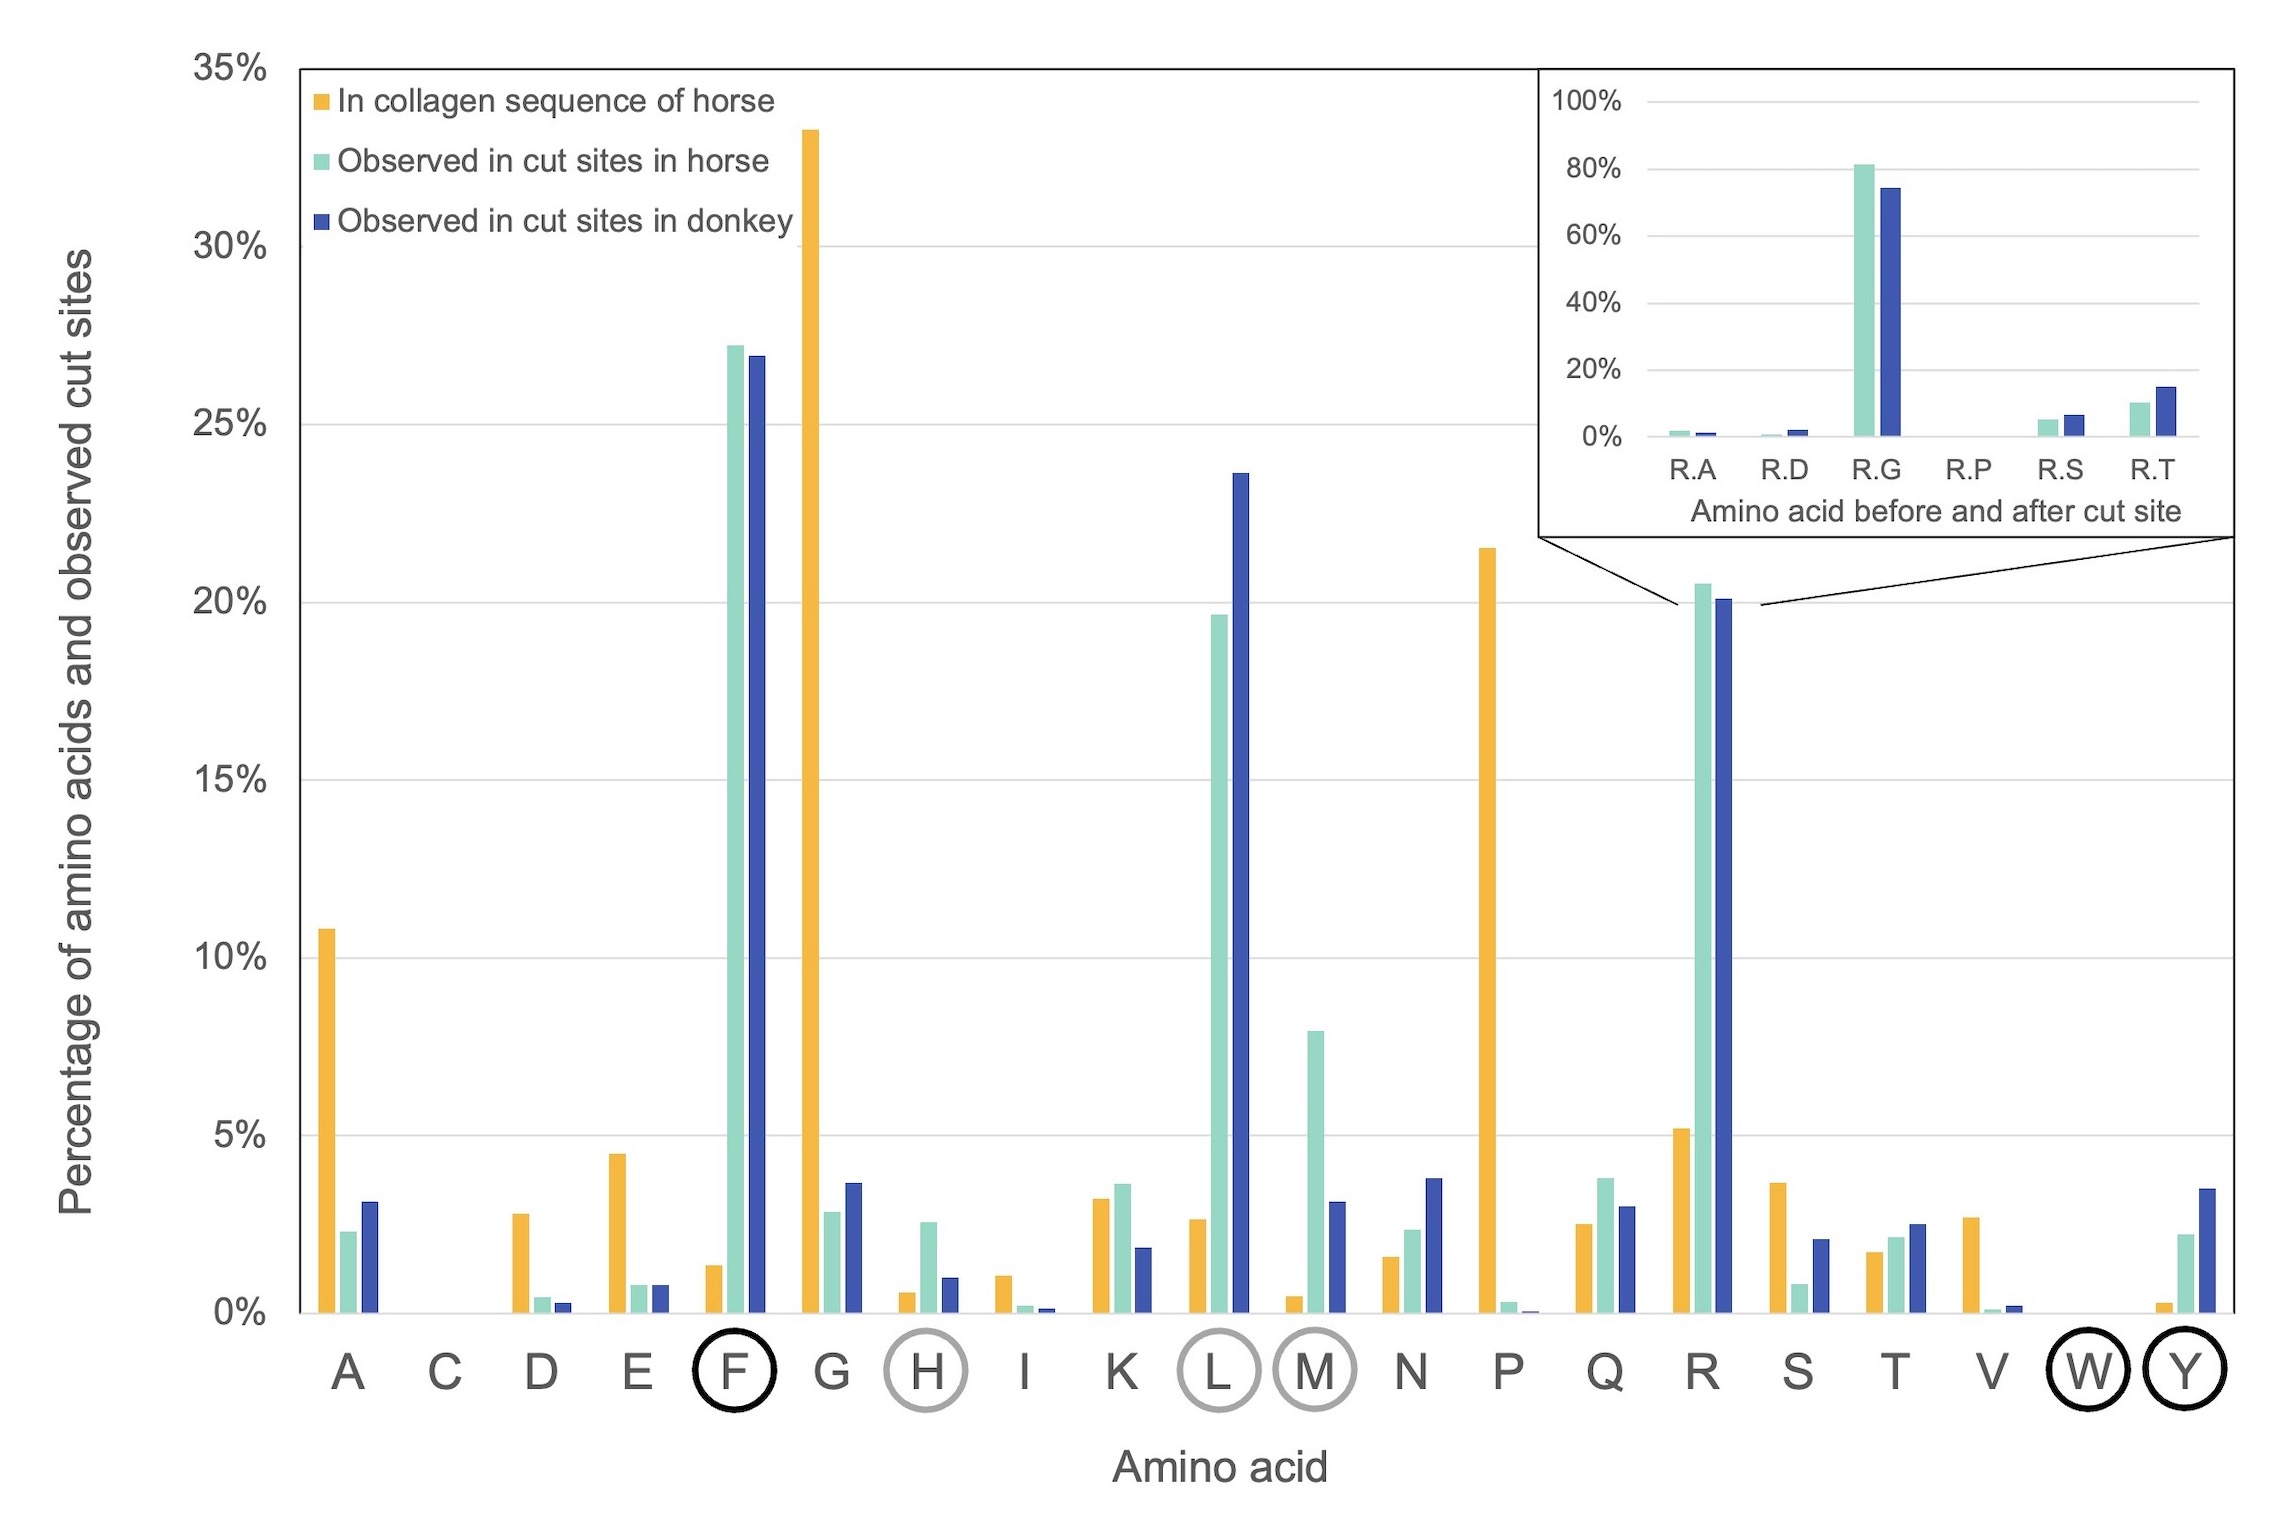
\includegraphics[width=1\linewidth]{../img/chymocutsite} \caption{\textcolor{blue}{Comparison of the percentage of amino acids in equid collagen (yellow) to the percentage of empirically observed cut sites at that amino acid in LC-MS/MS data (light blue, dark blue). The percentage of each amino acid in collagen is derived from the horse mature protein COL1A1 and COL1A2 sequences and calculated by Protein Calculator} (Anthis and Clore, 2013). \textcolor{blue}{Whether a given amino acid is located at a primary (black) or secondary (gray) chymotrypsin cut site is indicated by circles. The inset shows the relative percentage of different N-terminal residues at arginine cut sites. }}\label{fig:chymocutplot}
\end{figure*}

Enzymatic digestion can be variable, with the probability of cutting at any one location based upon the buffer solution (Tipton et al., 2009), presence of cofactors (Broderick, 2001), the primary amino acid (Keil, 2012), amino acid composition up to six amino acids in either direction of the cut site (Keil, 2012), and the structure of the protein (Hartley, 1960). This is commonly seen in ZooMS with trypsin. Trypsin cuts primarily at the C-terminal side of arginine and lysine but often does not cut when a proline follows the arginine or lysine in the sequence (Olsen et al., 2004; Rodriguez et al., 2008). Some of the standard ZooMS markers are based on these predictable missed cleavages due to the presence of a proline (Buckley et al., 2009; Keil, 2012; Welker et al., 2016). Chymotrypsin activity has been thoroughly investigated (Keil, 2012). Chymotrypsin cuts at the C-terminal side of tyrosine, phenylalanine, and tryptophan, and with lower efficiency at the C-terminal side of leucine, methionine, and histidine. Cleavages on the C-terminal side of arginine are also possible although rare (Keil, 2012). Nevertheless, we do observe multiple cleavages C-terminal to arginine during chymotrypsin digestion of equid COL1\textcolor{blue}{, which could correspond to an atypical cleavage of chymotrypsin or the presence of trypsin co-purified with chymotrypsin}.

In \textcolor{blue}{the case of an atypical cleavage}, the following factors increase the likelihood of cleavage at this particular arginine. \textcolor{blue}{First, COL1 collagen has a low number of preferential chymotrypsin cut sites, tyrosine, phenylalanine, and tryptophan, because these large amino acids destabilize the collagen triple helix} (Bella, 2016). These amino acids are largely absent from collagen and represent only 34/2072 amino acids in equid COL1A1 and COL1A2 (Figure \ref{fig:chymocutplot}). \textcolor{blue}{Although chymotrypsin has secondary cut site activity C-terminal to lysine, methionine, and histidine, these amino acids also have low abundance in collagen, representing 77/2072 amino acids in equid COL1A1 and COL1A2 (Figure \ref{fig:chymocutplot}).} Therefore, non-preferential cleavage sites are more commonly seen (Gattiker et al., 2002). Second, the sequence around the cleavage is GP\textbf{R}GRT. The three amino acids around the cleavage site are known to impact the success of cleavage for chymotrypsin, especially when the affinity to the primary amino acid (in this case the arginine before the cut site) is low (Keil, 2012). Both amino acid and location impact that success. For example, although a proline directly after an arginine inhibits cleavage by trypsin, a proline before an arginine increases the likelihood of cleavage by chymotrypsin. Also increasing the likelihood of cleavage after this particular arginine are the glycine in the first position after the cut site and the arginine in the second position after the cut site (Gibson and Dixon, 1969; Keil, 2012, 1987).

\textcolor{blue}{Alternatively, small amounts of residual trypsin can be present within commercially prepared chymotrypsin obtained by enzyme purification (\emph{pers comm} Promega technical support). Such low-level residual trypsin activity cannot be excluded as a possible contributor to cleavage at arginine residues. However, when analysing the remaining LC-MS/MS data using both semi-specific to chymotrypsin and non-specific enzyme parameters, the protein chymotrypsin was identified but trypsin was not identified at 1\% protein FDR. For the semi-specific search all of the peptides identified to chymotrypsin with a PEP 2D score less than 0.001 were searched against the NCBI protein database using BlastP and were specifically searched against trypsin and no identity to trypsin was found for any of the identified peptides.}

\textcolor{blue}{LC-MS/MS analysis of our chymotrypsin digestions revealed that cleavage was elevated after (C-terminal to) the few tyrosine and phenylalanine residues present in collagen (Table S3). Cleavage also occurred C-terminal to lysine and methionine when they were not followed by a proline inhibiting enzyme binding. Combined the primary and secondary cut sites accounted for 59\% of the observed cut sites. The most common non-preferential cleavage site in both COL1A1 and COL1A2 was found to be C-terminal to an arginine, accounting for about 20\% of the observed cut sites (Figure \ref{fig:chymocutplot}). Of those cut sites at arginine, cases where the cut site is between arginine and glycine make up 70-80\% (Figure \ref{fig:chymocutplot}, insert). When scaling against the number of the particular amino acid residues in the collagen sequence, the most frequent cut sites were C-terminal to phenylalanine, methionine, tyrosine, and lysine, followed by arginine and histidine. Although proline and glycine make up a large percentage of the overall amino acid composition, scaled values indicate that proportionally very few of the cut sites occurred C-terminal to proline or glycine, as predicted. (Table S3). When comparing horse and donkey MALDI spectra, we confirm that the marker peaks at \emph{m/z} 2497 and \emph{m/z} 2511 correspond to collagen amino acid differences between these two species and allow robust taxonomic discrimination.}

\begin{landscape}\begin{table}

\caption{\label{tab:eqtable3}Sample list of all archaeological and taxonomic reference samples analysed in this study.}
\centering
\fontsize{7}{9}\selectfont
\begin{tabular}[t]{cccccc>{}c>{}c}
\toprule
Sample ID & Lab Code & Site & Country & Time Period & Skeletal Element & Morphological Id. & ZooMS Id.\\
\midrule
TRAOF100 & HZ145 & Troia & Portugal & Roman & Left Femur & \em{Equus asinus} & \em{Equus asinus}\\
TRAOF101 & HZ146 & Troia & Portugal & Roman & Left Scapula & \em{Equus asinus} & \em{Equus asinus}\\
TRAOF102 & HZ147 & Troia & Portugal & Roman & Mandible & \em{Equus asinus} & \em{Equus asinus}\\
TRAOF104 & HZ149 & Troia & Portugal & Roman & Pelvis & \em{Equus asinus} & \em{Equus asinus}\\
TRAOF105 & HZ150 & Troia & Portugal & Roman & Rib & \em{Equus {\normalfont sp.}} & \em{Equus asinus}\\
TRAOF107 & HZ152 & Troia & Portugal & Roman & Long bone fragment & \em{Equus {\normalfont sp.}} & \em{Equus asinus}\\
RDA.19.EQ1 & HZ156 & Rua do Anjos & Portugal & Roman & Molar & \em{Equus {\normalfont sp.}} & \em{Equus asinus}\\
RDA.19.EQ2 & HZ157 & Rua do Anjos & Portugal & Roman & Molar & \em{Equus {\normalfont sp.}} & \em{Equus caballus}\\
RDA.19.EQ3 & HZ158 & Rua do Anjos & Portugal & Roman & Mandible & \em{Equus {\normalfont sp.}} & \em{Equus caballus}\\
RDA.19.EQ4 & HZ159 & Rua do Anjos & Portugal & Roman & Metapodial & \em{Equus {\normalfont sp.}} & \em{Equus caballus}\\
RDA.19.EQ5 & HZ160 & Rua do Anjos & Portugal & Roman & Metapodial & \em{Equus {\normalfont sp.}} & \em{Equus caballus}\\
RDA.19.EQ7 & HZ161 & Rua do Anjos & Portugal & Roman & Radius & \em{Equus {\normalfont sp.}} & \em{Equus caballus}\\
RDA.19.EQ8 & HZ162 & Rua do Anjos & Portugal & Roman & Pelvis & \em{Equus {\normalfont sp.}} & \em{Equus caballus}\\
RDA.19.EQ9 & HZ163 & Rua do Anjos & Portugal & Roman & Astragalus & \em{Equus {\normalfont sp.}} & \em{Equus asinus}\\
RDA.19.EQ10 & HZ164 & Rua do Anjos & Portugal & Roman & Femur & \em{Equus {\normalfont sp.}} & \em{Equus caballus}\\
LCB.15.EQ19 & HZ153 & Largo do Coutador & Portugal & Late Antiquity & Metapodial & \em{Equus {\normalfont sp.}} & \em{Equus asinus}\\
LCB.15.EQ18 & HZ154 & Largo do Coutador & Portugal & Late Antiquity & Molar & \em{Equus {\normalfont sp.}} & \em{Equus asinus}\\
LCB.15.EQ17 & HZ155 & Largo do Coutador & Portugal & Late Antiquity & Molar & \em{Equus {\normalfont sp.}} & \em{Equus asinus}\\
RNA63EQ11 & HZ165 & Rua Nova do Almada 63 & Portugal & Roman Imperial & Molar & \em{Equus {\normalfont sp.}} & \em{Equus caballus}\\
RNA63EQ12 & HZ166 & Rua Nova do Almada 63 & Portugal & Roman Imperial & Incisor & \em{Equus {\normalfont sp.}} & \em{Equus asinus}\\
BPLX.246 & HZ167 & Banco de Portugal & Portugal & Roman & Cranium & \em{Equus {\normalfont sp.}} & \em{Equus asinus}\\
H4.1070.1 & HZ143 & Los Morrones 11 & Spain & Iron Age & Radius & \em{Equus caballus} & \em{Equus caballus}\\
H4.1070.2 & HZ144 & Los Morrones 12 & Spain & Iron Age & Radius & \em{Equus caballus} & \em{Equus caballus}\\
H4.1075.3 & PHD1075.3 & Los Morrones 11 & Spain & Iron Age & Radius & \em{Equus caballus} & \em{Equus caballus}\\
TRSLOF100 & HZ140 & Torre Sal & Spain & Iberian & Radius & \em{Equus caballus} & \em{Equus caballus}\\
TRSLOF103 & PHDTSOF100 & Torre Sal & Spain & Iberian & Radius & \em{Equus caballus} & \em{Equus caballus}\\
MJV.1 & HZ121 & Horta da Torre & Portugal & Late Roman & Right Radius & \em{Equus caballus} & \em{Equus caballus}\\
MJV.2 & HZ122 & Horta da Torre & Portugal & Late Roman & Right Metacarpus & \em{Equus caballus} & \em{Equus caballus}\\
MJV.3 & HZ123 & Cacela - Po\c{c}o Antigo & Portugal & Late Medieval Islamic & Calcaneum R & \em{Equus {\normalfont sp.}} & \em{Equus caballus}\\
MJV.5 & HZ125 & Cacela - Largo Fortaleza & Portugal & Late Medieval Islamic/Christian & Upper Incisor 1 or 2 R (root) & \em{Equus {\normalfont sp.}} & \em{Equus asinus}\\
MJV.7 & HZ127 & Oficina Senhor Carrilho & Portugal & Medieval Islamic & Metapodial & \em{Equus {\normalfont sp.}} & \em{Equus caballus}\\
MJV.11 & HZ131 & Castillo de Aracena & Spain & Medieval Islamic & Scapula R & \em{Equus {\normalfont sp.}} & \em{Equus caballus}\\
MJV.12 & HZ132 & Castillo de Aracena & Spain & Late Medieval Islamic/Christian & Scapula L & \em{Equus {\normalfont sp.}} & \em{Equus asinus}\\
MJV.13 & HZ133 & Castillo de Aracena & Spain & Late Medieval Islamic/Christian & Scapula R & \em{Equus {\normalfont sp.}} & \em{Equus caballus}\\
MJV.14 & HZ134 & Rua da S\'{e} & Portugal & Medieval Islamic & Ulna L & \em{Equus caballus} & \em{Equus caballus}\\
\textbf{MJV.15} & \textbf{HZ135} & \textbf{Rua da S\'{e}} & \textbf{Portugal} & \textbf{Medieval Islamic} & \textbf{Humerus R} & \textbf{\em{Equus {\normalfont sp.}}} & \textbf{\em{Equus asinus}}\\
MJV.16 & HZ136 & Convento das Bernardas & Portugal & Late Modern (18/19th century) & Cranium & \em{Equus caballus} & \em{Equus caballus}\\
MJV.17 & HZ137 & Cerro da Vila & Portugal & Roman Imperial & Metacarpus L & \em{Equus {\normalfont sp.}} & \em{Equus asinus}\\
MJV.18 & HZ138 & Cerro da Vila & Portugal & Roman Imperial & Ulna R & \em{Equus {\normalfont sp.}} & \em{Equus asinus}\\
MJV.19 & HZ139 & Cerro da Vila & Portugal & Roman Imperial & Maxillar & \em{Equus caballus} & \em{Equus caballus}\\
LARC.265 & PHD265 & Minho & Portugal & Modern/Reference & Vertebra & \em{Equus caballus} & \em{Equus caballus}\\
LARC.238 & PHD238 & Minho & Portugal & Modern/Reference & Nasal conchae & \em{Equus caballus} & \em{Equus caballus}\\
LARC.2324 & PHD2324 & Minho & Portugal & Modern/Reference & Scapula & \em{Equus caballus} & \em{Equus caballus}\\
LARC.1498 & PHD1498 & Baixo Alentejo & Portugal & Modern/Reference & Vertebra & \em{Equus asinus} & \em{Equus asinus}\\
LARC.2000 & PHD2000 & Tr\'{a}s-os-Montes & Portugal & Modern/Reference & Vertebra & \em{Equus asinus} & \em{Equus asinus}\\
LARC.2313 & PHD2313 & Tr\'{a}s-os-Montes & Portugal & Modern/Reference & Vertebra & \em{Equus asinus} & \em{Equus asinus}\\
\bottomrule
\multicolumn{8}{l}{\rule{0pt}{1em}\textit{Note: }}\\
\multicolumn{8}{l}{\rule{0pt}{1em}The entry in bold was formally identified as an equid but presumed to be horse since all the other equids from the same context were adult horses. But ZooMS identification revealed it to be a donkey.}\\
\end{tabular}
\end{table}
\end{landscape}

\hypertarget{modern-and-archaeological-samples}{%
\subsection{Modern and Archaeological samples}\label{modern-and-archaeological-samples}}



\begin{figure*}

{\centering 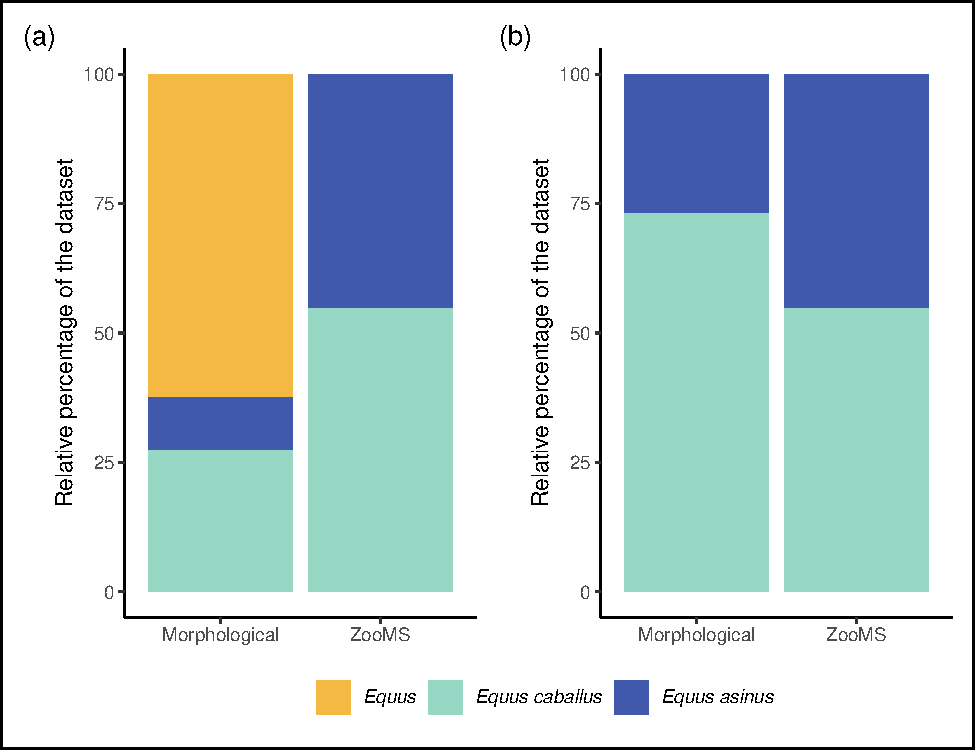
\includegraphics[width=0.70\textwidth]{equid_main_files/figure-latex/resultbarplotr-1} 

}

\caption{Taxonomic assignment of 40 archaeological \emph{Equus} skeletal remains using conventional morphological and ZooMS techniques. (a) Morphological analysis results in a high proportion (62.5\%) of bones that cannot be reliably classified below the level of genus (\emph{Equus}), whereas all bones could be identified to the species level (\emph{E. caballus} or \emph{E. asinus}) using ZooMS. (b) Taxonomic analyses based only on bones identifiable to species result in discrepant estimations of the relative abundance of horses and donkeys depending on the identification method. Morphological analysis appears to under-identify donkeys, potentially introducing bias into downstream analyses.}\label{fig:resultbarplotr}
\end{figure*}

The geographical origin and time period of the samples analysed in this study are presented in Table \ref{tab:eqtable3}.
Taxonomic reference samples from the Laboratório de Arqueociências (Direção Geral do Património Cultural, Lisbon) mammal collection produced high quality tryptic and chymotryptic digests. The tryptic digest spectra were used to confirm that the samples were indeed equids using the presence of previously reported \emph{Equus} marker peaks (SI\textcolor{blue}{1}) (Welker et al., 2016). All of the archaeological samples (n = 40) analysed had sufficient collagen preservation to allow taxonomic identification as \emph{Equus}, in case of tryptic digests, and as either horse or donkey, in the case of chymotryptic digests (Figure \ref{fig:equidmarkerplot} \textbf{(b)}). Of the 40 archaeological bone specimens, traditional morphological analyses identified 25 as \emph{Equus} sp., 11 specimens as horses, and 4 as donkeys. Using the new collagen marker, we could unambiguously distinguish all samples as either horse (n = 22) or donkey (n = 18). Of the 15 \emph{Equus} specimens assigned to the species level based on morphological criteria, the ZooMS identification was in agreement for all but one (Table \ref{tab:eqtable3}, Figure \ref{fig:resultbarplotr} \textbf{(a)}). The sample MJV.15, a neonatal individual, was presumed to be a horse but formally identified just as an equid, as morphologically there are no criteria to distinguish neonatal equids. This assumption was based on the fact that the other equid remains from the same context (Portuguese Medieval Islamic) were adult horses. But ZooMS identified the individual as a donkey (Table \ref{tab:eqtable3}, Figure \ref{fig:equidmarkerplot} \textbf{(b)}).

Because of the close evolutionary distance within Equidae (Orlando et al., 2013), sterile hybrids can be produced between horses and donkeys: mules (\emph{Equus asinus}\(^{\male}\) x \emph{Equus caballus}\(^{\female}\)) and hinnies (\emph{Equus caballus}\(^{\male}\) x \emph{Equus asinus}\(^{\female}\)). Hybrids are both wild born and also intentionally bred for favourable characteristics such as enhanced strength and harder hooves. In designing the study, we attempted to exclude bones likely derived from hybrids, although that possibility cannot be excluded entirely. Hybrids are frequently difficult to distinguish in the archaeological record using either morphological characteristics or mtDNA, leaving nuclear DNA as the only entirely reliable indicator at present (Lepetz et al., 2021; Schubert et al., 2017; Sharif et al., 2022). \textcolor{blue}{Yet, the importance of hybrids in the archaeological record is increasingly being better understood. Nuclear aDNA and the Zonkey Computational Pipeline on 873 archaeological equid bones from French sites dating from the Iron Age to Modern times identified 55 mules and 1 hinny. During the Roman Period, hybrids accounted for 20-34.5\% of the equid remains studied} (Lepetz et al., 2021). \textcolor{blue}{The same pattern is true for the Northern Alps where an aDNA study of 295 equid remains from the Roman Period identified 48 mules} (Sharif et al., 2022). \textcolor{blue}{Since} hybrids have copies of both horse and donkey COL1 genes, they should be identifiable by ZooMS. Therefore, further characterisation of this ZooMS marker which separates horses and donkeys in both other species of equids (wild asses and zebras) and equid hybrids will be important.

The archaeological bones in this study were chosen because they were well preserved with enough morphological characteristics to be able to be identified to at least genus level across a wide spatial-temporal range in Western Iberia. The successful application of a new ZooMS marker to this sample set showcases the ability of ZooMS to now distinguish between domestic equid species. In addition, because ZooMS increases the proportion of taxonomically identified bones, it reduces bias in the analysis due to missing data. For example, in comparing taxonomic profiles obtained for this sample set, we observed that morphological analysis tends to under-identify donkeys, resulting in inflated estimations of the relative abundance of horses (Figure \ref{fig:resultbarplotr} (b)). \textcolor{blue}{This marker opens the ability to increase the resolution for ZooMS on assemblages that are often less well identified} (Welker et al., 2016) \textcolor{blue}{in a two-step process. Collagen can be extracted from faunal remains and digested with trypsin for identification using standard ZooMS markers. For samples identified as equid, the remaining extracted collagen can be digested with chymotrypsin for species identification. The results from this two-step process can then be integrated into traditional zooarchaeological frameworks} (Brandt et al., 2014; Brown et al., 2021b; Harvey et al., 2018).

\hypertarget{conclusion}{%
\section{Conclusion}\label{conclusion}}

\textcolor{blue}{Using the enzyme chymotrypsin, we have developed a ZooMS marker which can reliably distinguish between domestic horse and donkey.} As this is the first use of an enzyme other than trypsin for ZooMS on archaeological \textcolor{blue}{faunal} material, we propose an approach for suspected equids in which collagen extracts are split into two fractions and digested separately, first with trypsin for confirmation of \emph{Equus} genus using the standard ZooMS markers, and then with chymotrypsin to distinguish domestic horse and donkey. The ability to quickly and easily discriminate domestic horses and donkeys using ZooMS is highly valuable for zooarchaeological studies as these species are often indistinguishable morphologically, but are treated economically and culturally very differently.

\hypertarget{supporting-information}{%
\section*{Supporting Information}\label{supporting-information}}
\addcontentsline{toc}{section}{Supporting Information}

Supplementary Information File (PDF)

\hypertarget{acknowledgements}{%
\section*{Acknowledgements}\label{acknowledgements}}
\addcontentsline{toc}{section}{Acknowledgements}

We would like to thank Vanessa Naverette Belda (Universidade de Évora), Ana Beatriz Santos (Uniarq, Universidade de Lisboa), and Mariana Nabais (Uniarq, Universidade de Lisboa) for providing samples for the study, Sunia A.Trauger and Renee A. Robinson at the Harvard Center for Mass Spectrometry for technical assistance, and Andrew Cepeda and Chris Paul for logistical support. The authors would also like to thank Simon Davis and Carlos Pimenta whose efforts have resulted in the taxonomic reference collection at Laboratório de Arqueociências (Direção Geral do Património Cultural, Lisbon). R.P thanks Silvia Russo for help in finding colour-blind friendly palette for data visualisation. R.P and C.B.D have received funding from the European Union's Horizon 2020 research and innovation programme under the Marie Skłodowska-Curie grant agreement No.~766311. C.W is supported by the European Research Council under the European Union's Horizon 2020 Research and Innovation Program Grant 804884-DAIRYCULTURES, the Werner Siemens Stiftung (``Paleobiotechnology''), the Max Planck--Harvard Research Center for the Archaeoscience of the Ancient Mediterranean, and Harvard University. C.D. is funded by the Science and Technology Foundation in Portugal through the project BRoman (Ref. PTDC/HAR-ARQ/4909/2020).

\hypertarget{references}{%
\section*{References}\label{references}}
\addcontentsline{toc}{section}{References}

\hypertarget{refs}{}
\begin{CSLReferences}{1}{0}
\leavevmode\vadjust pre{\hypertarget{ref-albizuri_nadal91}{}}%
Albizuri, S., Nadal, J., 1991. Estudi de l'èquid aparegut en relació amb l'estructura {E10} de l'{Hort} d'en {Grimau}. Olerdulae 3, 112--117.

\leavevmode\vadjust pre{\hypertarget{ref-aleixo18}{}}%
Aleixo, P.A. da S., 2018. Estudo zooarqueológico do sítio do {Neolítico Final} do {Barranco} do {Xacafre}, {Ferreira} do {Alentejo}.

\leavevmode\vadjust pre{\hypertarget{ref-ameen_etal21}{}}%
Ameen, C., Benkert, H., Fraser, T., Gordon, R., Holmes, M., Johnson, W., Lauritsen, M., Maltby, M., Rapp, K., Townend, T., Baker, G.P., Jones, L.M., Vo Van Qui, C., Webley, R., Liddiard, R., Sykes, N., Creighton, O.H., Thomas, R., Outram, A.K., 2021. In search of the {``great horse''}: {A} zooarchaeological assessment of horses from {England} ({AD} 300--1650). International Journal of Osteoarchaeology 31, 1247--1257. \url{https://doi.org/10.1002/oa.3038}

\leavevmode\vadjust pre{\hypertarget{ref-anthis_clore13}{}}%
Anthis, N.J., Clore, G.M., 2013. Sequence‐specific determination of protein and peptide concentrations by absorbance at 205 nm. Protein Science 22, 851--858. \url{https://doi.org/10.1002/pro.2253}

\leavevmode\vadjust pre{\hypertarget{ref-arloing82}{}}%
Arloing, J., 1882. Caractères ostéologiques différentiels de l'âne, du cheval et de leurs hybrides.

\leavevmode\vadjust pre{\hypertarget{ref-armitage_chapman79}{}}%
Armitage, P.L., Chapman, H., 1979. Roman mules. {London Archaeologist Association}.

\leavevmode\vadjust pre{\hypertarget{ref-azzaroli78}{}}%
Azzaroli, A., 1978. On a {Late Pleistocene Ass} from {Tuscany}\textbar{} with {Notes} on the {History} of {Asses}. Palaeontographia Italica Pisa 71, 27--47.

\leavevmode\vadjust pre{\hypertarget{ref-baxter98}{}}%
Baxter, I.L., 1998. Species identification of equids from {Western European} archaeological deposits: Methodologies, techniques and problems. Current and Recent Research in Osteoarchaeology. Oxbow, Oxford 16.

\leavevmode\vadjust pre{\hypertarget{ref-beja-pereira_etal04}{}}%
Beja-Pereira, A., England, P.R., Ferrand, N., Jordan, S., Bakhiet, A.O., Abdalla, M.A., Mashkour, M., Jordana, J., Taberlet, P., Luikart, G., 2004. African {Origins} of the {Domestic Donkey}. Science 304, 1781--1781. \url{https://doi.org/10.1126/science.1096008}

\leavevmode\vadjust pre{\hypertarget{ref-bella16}{}}%
Bella, J., 2016. Collagen structure: New tricks from a very old dog. Biochemical Journal 473, 1001--1025.

\leavevmode\vadjust pre{\hypertarget{ref-brandt_etal14}{}}%
Brandt, L.Ø., Schmidt, A.L., Mannering, U., Sarret, M., Kelstrup, C.D., Olsen, J.V., Cappellini, E., 2014. Species {Identification} of {Archaeological Skin Objects} from {Danish Bogs}: {Comparison} between {Mass Spectrometry-Based Peptide Sequencing} and {Microscopy-Based Methods}. PLOS ONE 9, e106875. \url{https://doi.org/10.1371/journal.pone.0106875}

\leavevmode\vadjust pre{\hypertarget{ref-broderick01}{}}%
Broderick, J., 2001. Coenzymes and cofactors, in: {eLS}. {John Wiley \& Sons, Ltd}. \url{https://doi.org/10.1038/npg.els.0000631}

\leavevmode\vadjust pre{\hypertarget{ref-brown_etal21}{}}%
Brown, S., Douka, K., Collins, M.J., Richter, K.K., 2021a. On the standardization of {ZooMS} nomenclature. Journal of Proteomics 235, 104041. \url{https://doi.org/10.1016/j.jprot.2020.104041}

\leavevmode\vadjust pre{\hypertarget{ref-brown_etal20}{}}%
Brown, S., Hebestreit, S., Wang, N., Boivin, N., Douka, K., Richter, K., 2022. Zooarchaeology by {Mass Spectrometry} ({ZooMS}) for bone material - {AmBiC} protocol protocol metadata {[}WWW Document{]}. URL \url{https://dx.doi.org/10.17504/protocols.io.bffdjji6}

\leavevmode\vadjust pre{\hypertarget{ref-brown_etal21a}{}}%
Brown, S., Wang, N., Oertle, A., Kozlikin, M.B., Shunkov, M.V., Derevianko, A.P., Comeskey, D., Jope-Street, B., Harvey, V.L., Chowdhury, M.P., Buckley, M., Higham, T., Douka, K., 2021b. Zooarchaeology through the lens of collagen fingerprinting at {Denisova Cave}. Scientific Reports 11, 15457. \url{https://doi.org/10.1038/s41598-021-94731-2}

\leavevmode\vadjust pre{\hypertarget{ref-buckley_collins11}{}}%
Buckley, M., Collins, M.J., 2011. Collagen survival and its use for species identification in {Holocene-lower Pleistocene} bone fragments from {British} archaeological and paleontological sites. Antiqua 1, e1--e1. \url{https://doi.org/10.4081/antiqua.2011.e1}

\leavevmode\vadjust pre{\hypertarget{ref-buckley_etal09}{}}%
Buckley, M., Collins, M., Thomas‐Oates, J., Wilson, J.C., 2009. Species identification by analysis of bone collagen using matrix-assisted laser desorption/ionisation time-of-flight mass spectrometry. Rapid Communications in Mass Spectrometry 23, 3843--3854. \url{https://doi.org/10.1002/rcm.4316}

\leavevmode\vadjust pre{\hypertarget{ref-buckley_etal17}{}}%
Buckley, M., Harvey, V.L., Chamberlain, A.T., 2017. Species identification and decay assessment of {Late Pleistocene} fragmentary vertebrate remains from {Pin Hole Cave} ({Creswell Crags}, {UK}) using collagen fingerprinting. Boreas 46, 402--411. \url{https://doi.org/10.1111/bor.12225}

\leavevmode\vadjust pre{\hypertarget{ref-cardoso95}{}}%
Cardoso, J.L., 1995. Os ídolos falange do povoado pré-histórico de {Leceia} ({Oeiras}): Estudo comparado. Estudos Arqueológicos de Oeiras 5.

\leavevmode\vadjust pre{\hypertarget{ref-cardoso94}{}}%
Cardoso, J.L., 1994. A {Fauna} de mamíferos da época {Muçulmana} das {Mesas} do {Castelinho} ({Almodôvar}): {Materiais} das {Campanhas} de 1989-1992. Arqueologia Medieval 201--220.

\leavevmode\vadjust pre{\hypertarget{ref-cardoso93}{}}%
Cardoso, J.L., 1993. Restos de grandes mamíferos da ilha do {Pessegueiro}: Contribuição para o conhecimento da alimentação na {Época Romana}. Ilha do Pessegueiro: porto romano da Costa Alentejana 205--215.

\leavevmode\vadjust pre{\hypertarget{ref-cardoso_detry02}{}}%
Cardoso, J.L., Detry, C., 2002. Estudo arqueozoológico dos restos de ungulados do povoado pré-histórico de {Leceia} ({Oeiras}). Estudos Arqueológicos de Oeiras 10, 131--182.

\leavevmode\vadjust pre{\hypertarget{ref-cardoso_etal13}{}}%
Cardoso, J.L., Vilstrup, J.T., Eisenmann, V., Orlando, L., 2013. First evidence of {Equus} asinus {L}. In the {Chalcolithic} disputes the {Phoenicians} as the first to introduce donkeys into the {Iberian Peninsula}. Journal of Archaeological Science 40, 4483--4490. \url{https://doi.org/10.1016/j.jas.2013.07.010}

\leavevmode\vadjust pre{\hypertarget{ref-castanos05}{}}%
Castaños, P.M., 2005. Estudio de la fauna de {Cueva Mayor} de {Atapuerca}, in: Estudios Sobre {Atapuerca} ({Burgos}). {Servicio de Publicaciones= Argitalpen Zerbitzua}, pp. 247--258.

\leavevmode\vadjust pre{\hypertarget{ref-chuang_bonhomme19}{}}%
Chuang, R., Bonhomme, V., 2019. Rethinking the dental morphological differences between domestic equids. Journal of Archaeological Science 101, 140--148. \url{https://doi.org/10.1016/j.jas.2018.02.020}

\leavevmode\vadjust pre{\hypertarget{ref-clutton-brock92}{}}%
Clutton-Brock, J., 1992. Horse power: A history of the horse and the donkey in human societies. {Harvard University Press}.

\leavevmode\vadjust pre{\hypertarget{ref-coutu_etal21}{}}%
Coutu, A., Taurozzi, A.J., Mackie, M., Jensen, T.Z.T., Collins, M.J., Sealy, J., 2021. Palaeoproteomics confirm earliest domesticated sheep in southern {Africa} ca. 2000 {BP}. Sci Rep 11, 6631. \url{https://doi.org/10.1038/s41598-021-85756-8}

\leavevmode\vadjust pre{\hypertarget{ref-cucchi_etal}{}}%
Cucchi, T., Mohaseb, A., Peigné, S., Debue, K., Orlando, L., Mashkour, M., 2017. Detecting taxonomic and phylogenetic signals in equid cheek teeth: Towards new palaeontological and archaeological proxies. Royal Society Open Science 4, 160997. \url{https://doi.org/10.1098/rsos.160997}

\leavevmode\vadjust pre{\hypertarget{ref-davis06}{}}%
Davis, S., 2006. Faunal remains from {Alcáçova} de {Santarém}. Portugal, Instituto português de arqueologia.

\leavevmode\vadjust pre{\hypertarget{ref-davis02}{}}%
Davis, S., 2002. The mammals and birds from the {Gruta} do {Caldeirão}, {Portugal}. Revista Portuguesa de Arqueologia 5, 29--98.

\leavevmode\vadjust pre{\hypertarget{ref-davis_etal08}{}}%
Davis, S., Gonçalves, M.J., Gabriel, S., 2008. Animal remains from a {Moslem} period (12th/13th century {AD}) lixeira (garbage dump) in {Silves}, {Algarve}, {Portugal}. Revista portuguesa de Arqueologia 11, 183--258.

\leavevmode\vadjust pre{\hypertarget{ref-davis80}{}}%
Davis, S.J., 1980. Late {Pleistocene} and {Holocene} equid remains from {Israel}. Zoological Journal of the Linnean Society 70, 289--312.

\leavevmode\vadjust pre{\hypertarget{ref-davis_etal18}{}}%
Davis, S.J., Gabriel, S., Simões, T., 2018. Animal remains from {Neolithic Lameiras}, {Sintra}: The earliest domesticated sheep, goat, cattle and pigs in {Portugal} and some notes on their evolution. Archaeofauna-Madrid- 27, 93--172.

\leavevmode\vadjust pre{\hypertarget{ref-davis_goncalves17}{}}%
Davis, S.J., Gonçalves, A., 2017. Animal remains from the 4th--5th century {AD} well at {São Miguel} de {Odrinhas}, {Sintra}, {Portugal}: Tiny sheep and a dwarf dog. Revista portuguesa de arqueologia 20, 139--156.

\leavevmode\vadjust pre{\hypertarget{ref-detry07}{}}%
Detry, C., 2007. Paleoecologia e {Paleoeconomia} do {Baixo Tejo} no {Mesolítico Final}: {O} contributo do estudo dos mamíferos dos concheiros de {Muge}. {Universidad de Salamanca}.

\leavevmode\vadjust pre{\hypertarget{ref-detry_arruda13}{}}%
Detry, C., Arruda, A.M., 2013. A fauna da {Idade} do {Ferro} e da {Época Romana} de {Monte Molião} ({Lagos}, {Algarve}): Continuidades e rupturas na dieta alimentar. Revista Portuguesa de Arqueologia 213--226.

\leavevmode\vadjust pre{\hypertarget{ref-detry_etal16}{}}%
Detry, C., Cardoso, J.L., Bugalhão, J., 2016. A alimentação em lisboa no decurso da idade do ferro : Resultados das escavações realizadas no núcleo arqueológico da rua dos correeiros (lisboa, portugal). SPAL. Revista de Prehistoria y Arqueología de la Universidad de Sevilla 67--82. \url{https://doi.org/10.12795/spal.2016i25.03}

\leavevmode\vadjust pre{\hypertarget{ref-detry_fabiao21}{}}%
Detry, C., Fabião, C., 2021. O cavalo na {Lisboa} romana. Lisboa romana, Felicitas Iulia Olisipo: A cidade produtora (e consumidora) 87--91.

\leavevmode\vadjust pre{\hypertarget{ref-detry_pimenta17}{}}%
Detry, C., Pimenta, J., 2017. Animal remains from medieval and modern {Vila Franca} de {Xira}, {Portugal}: {Excavations} at the {Neo-Realism Museum}. Cira Arqueologia 5, 238--259.

\leavevmode\vadjust pre{\hypertarget{ref-eisenmann86}{}}%
Eisenmann, V., 1986. Comparative osteology of modern and fossil horses, half-asses, and asses. Equids in the ancient world 1, 67--116.

\leavevmode\vadjust pre{\hypertarget{ref-eisenmann81}{}}%
Eisenmann, V., 1981. Etude des dents jugales inférieures des {Equus} ({Mammalia}, {Perissodactyla}) actuels et fossiles. Palaeovertebrata: revue trimestrielle de paléontologie des vertébrés 10, 130.

\leavevmode\vadjust pre{\hypertarget{ref-eisenmann80}{}}%
Eisenmann, V., 1980. Les chevaux ({Equus} sensu lato) fossiles et actuels: Crânes et dents jugales supérieures. {Éditions du Centre national de la recherche scientifique}.

\leavevmode\vadjust pre{\hypertarget{ref-eisenmann_beckouche86}{}}%
Eisenmann, V., Beckouche, S., 1986. Identification and discrimination of metapodials from {Pleistocene} and modern {Equus}, wild and domestic. Beihefte zum Tübinger Atlas des Vorderen Orients. Reihe A, Naturwissenschaften 19, 117.

\leavevmode\vadjust pre{\hypertarget{ref-forest08}{}}%
Forest, V., 2008. Equidés de la tène finale et de la période romaine en gaule: Approche ostéométrique. L'exploitation agricole dans son environnement à la fin de l'Âge du Fer: Nouvelles approches méthodologiques. Presented at the Rencontre de Saint-Julien: 18-19 novembre 2004 61--71.

\leavevmode\vadjust pre{\hypertarget{ref-gasteiger_etal05}{}}%
Gasteiger, E., Hoogland, C., Gattiker, A., Wilkins, M.R., Appel, R.D., Bairoch, A., 2005. Protein identification and analysis tools on the {ExPASy} server. The proteomics protocols handbook 571--607.

\leavevmode\vadjust pre{\hypertarget{ref-gattiker_etal02}{}}%
Gattiker, A., Bienvenut, W.V., Bairoch, A., Gasteiger, E., 2002. {FindPept}, a tool to identify unmatched masses in peptide mass fingerprinting protein identification. Proteomics 2, 1435--1444.

\leavevmode\vadjust pre{\hypertarget{ref-gibson_dixon69}{}}%
Gibson, D., Dixon, G., 1969. Chymotrypsin-like proteases from the sea anemone, {Metridium} senile. Nature 222, 753--756. \url{https://doi.org/10.1038/222753a0}

\leavevmode\vadjust pre{\hypertarget{ref-groves_mazak67}{}}%
Groves, C.P., Mazák, V., 1967. On some taxonomic problems of {Asiatic} wild asses; with the description of a new subspecies ({Perissodactyla}; {Equidae}). Zeitschrift für Säugetierkunde 32, 321--355.

\leavevmode\vadjust pre{\hypertarget{ref-hanot_bochaton18}{}}%
Hanot, P., Bochaton, C., 2018. New osteological criteria for the identification of domestic horses, donkeys and their hybrids in archaeological contexts. Journal of Archaeological Science 94, 12--20. \url{https://doi.org/10.1016/j.jas.2018.03.012}

\leavevmode\vadjust pre{\hypertarget{ref-hanot_etal17}{}}%
Hanot, P., Herrel, A., Guintard, C., Cornette, R., 2017. Morphological integration in the appendicular skeleton of two domestic taxa: The horse and donkey. Proceedings of the Royal Society B: Biological Sciences 284, 20171241. \url{https://doi.org/10.1098/rspb.2017.1241}

\leavevmode\vadjust pre{\hypertarget{ref-harrison_etal87}{}}%
Harrison, R.J., Moreno López, G., Legge, A.J., 1987. Moncín: Poblado prehistórico de la {Edad} del {Bronce} ({I}). Noticiario Arqueológico Hispánico (1979) 7--102.

\leavevmode\vadjust pre{\hypertarget{ref-hartley60}{}}%
Hartley, B., 1960. Proteolytic enzymes. Annual review of biochemistry 29, 45--72.

\leavevmode\vadjust pre{\hypertarget{ref-harvey_etal18}{}}%
Harvey, V.L., Daugnora, L., Buckley, M., 2018. Species identification of ancient {Lithuanian} fish remains using collagen fingerprinting. Journal of Archaeological Science 98, 102--111. \url{https://doi.org/10.1016/j.jas.2018.07.006}

\leavevmode\vadjust pre{\hypertarget{ref-janzen_etal21}{}}%
Janzen, A., Richter, K.K., Mwebi, O., Brown, S., Onduso, V., Gatwiri, F., Ndiema, E., Katongo, M., Goldstein, S.T., Douka, K., Boivin, N., 2021. Distinguishing {African} bovids using {Zooarchaeology} by {Mass Spectrometry} ({ZooMS}): {New} peptide markers and insights into {Iron Age} economies in {Zambia}. PLOS ONE 16, e0251061. \url{https://doi.org/10.1371/journal.pone.0251061}

\leavevmode\vadjust pre{\hypertarget{ref-jaworski_etal20}{}}%
Jaworski, K., Pankiewicz, A., Chrószcz, A., Poradowski, D., 2020. Different {Approach} to {Horses}---{The Use} of {Equid Remains} in the {Early Middle Ages} on the {Example} of {Ostrów Tumski} in {Wroclaw}. Animals 10, 2294. \url{https://doi.org/10.3390/ani10122294}

\leavevmode\vadjust pre{\hypertarget{ref-jonsson_etal14}{}}%
Jónsson, H., Schubert, M., Seguin-Orlando, A., Ginolhac, A., Petersen, L., Fumagalli, M., Albrechtsen, A., Petersen, B., Korneliussen, T.S., Vilstrup, J.T., Lear, T., Myka, J.L., Lundquist, J., Miller, D.C., Alfarhan, A.H., Alquraishi, S.A., Al-Rasheid, K.A.S., Stagegaard, J., Strauss, G., Bertelsen, M.F., Sicheritz-Ponten, T., Antczak, D.F., Bailey, E., Nielsen, R., Willerslev, E., Orlando, L., 2014. Speciation with gene flow in equids despite extensive chromosomal plasticity. Proceedings of the National Academy of Sciences 111, 18655--18660. \url{https://doi.org/10.1073/pnas.1412627111}

\leavevmode\vadjust pre{\hypertarget{ref-kearse_etal12}{}}%
Kearse, M., Moir, R., Wilson, A., Stones-Havas, S., Cheung, M., Sturrock, S., Buxton, S., Cooper, A., Markowitz, S., Duran, C., 2012. Geneious {Basic}: An integrated and extendable desktop software platform for the organization and analysis of sequence data. Bioinformatics 28, 1647--1649.

\leavevmode\vadjust pre{\hypertarget{ref-keil12}{}}%
Keil, B., 2012. Specificity of proteolysis. {Springer Science \& Business Media}.

\leavevmode\vadjust pre{\hypertarget{ref-keil87}{}}%
Keil, B., 1987. \href{https://www.ncbi.nlm.nih.gov/pubmed/3447153}{Proteolysis {Data Bank}: Specificity of alpha-chymotrypsin from computation of protein cleavages}. Protein Seq Data Anal 1, 13--20.

\leavevmode\vadjust pre{\hypertarget{ref-kimura_etal13}{}}%
Kimura, B., Marshall, F., Beja-Pereira, A., Mulligan, C., 2013. Donkey {Domestication}. Afr Archaeol Rev 30, 83--95. \url{https://doi.org/10.1007/s10437-012-9126-8}

\leavevmode\vadjust pre{\hypertarget{ref-p_kirby_etal13}{}}%
Kirby, D., Buckley, M., Promise, E., A. Trauger, S., Rose Holdcraft, T., 2013. Identification of collagen-based materials in cultural heritage. Analyst 138, 4849--4858. \url{https://doi.org/10.1039/C3AN00925D}

\leavevmode\vadjust pre{\hypertarget{ref-kunst00}{}}%
Kunst, G.K., 2000. Archaeozoological evidence for equid use, sex structure and mortality in a {Roman} auxiliary fort ({Carnuntum-Petronell}, lower {Austria}). Anthropozoologica 31, 109--118.

\leavevmode\vadjust pre{\hypertarget{ref-lepetz_etal21}{}}%
Lepetz, S., Clavel, B., Alioğlu, D., Chauvey, L., Schiavinato, S., Tonasso-Calvière, L., Liu, X., Fages, A., Khan, N., Seguin-Orlando, A., Der Sarkissian, C., Clavel, P., Estrada, O., Gaunitz, C., Aury, J.-M., Barme, M., Boulbes, N., Bourgois, A., Decanter, F., Foucras, S., Frère, S., Gardeisen, A., Jouanin, G., Méla, C., Morand, N., Nieto Espinet, A., Perdereau, A., Putelat, O., Rivière, J., Robin, O., Salin, M., Valenzuela-Lamas, S., Vallet, C., Yvinec, J.-H., Wincker, P., Orlando, L., 2021. Historical management of equine resources in {France} from the {Iron Age} to the {Modern Period}. Journal of Archaeological Science: Reports 40, 103250. \url{https://doi.org/10.1016/j.jasrep.2021.103250}

\leavevmode\vadjust pre{\hypertarget{ref-librado_etal21}{}}%
Librado, P., Khan, N., Fages, A., Kusliy, M.A., Suchan, T., Tonasso-Calvière, L., Schiavinato, S., Alioglu, D., Fromentier, A., Perdereau, A., Aury, J.-M., Gaunitz, C., Chauvey, L., Seguin-Orlando, A., Der Sarkissian, C., Southon, J., Shapiro, B., Tishkin, A.A., Kovalev, A.A., Alquraishi, S., Alfarhan, A.H., Al-Rasheid, K.A.S., Seregély, T., Klassen, L., Iversen, R., Bignon-Lau, O., Bodu, P., Olive, M., Castel, J.-C., Boudadi-Maligne, M., Alvarez, N., Germonpré, M., Moskal-del Hoyo, M., Wilczyński, J., Pospuła, S., Lasota-Kuś, A., Tunia, K., Nowak, M., Rannamäe, E., Saarma, U., Boeskorov, G., Lōugas, L., Kyselý, R., Peške, L., Bălășescu, A., Dumitrașcu, V., Dobrescu, R., Gerber, D., Kiss, V., Szécsényi-Nagy, A., Mende, B.G., Gallina, Z., Somogyi, K., Kulcsár, G., Gál, E., Bendrey, R., Allentoft, M.E., Sirbu, G., Dergachev, V., Shephard, H., Tomadini, N., Grouard, S., Kasparov, A., Basilyan, A.E., Anisimov, M.A., Nikolskiy, P.A., Pavlova, E.Y., Pitulko, V., Brem, G., Wallner, B., Schwall, C., Keller, M., Kitagawa, K., Bessudnov, A.N., Bessudnov, A., Taylor, W., Magail, J., Gantulga, J.-O., Bayarsaikhan, J., Erdenebaatar, D., Tabaldiev, K., Mijiddorj, E., Boldgiv, B., Tsagaan, T., Pruvost, M., Olsen, S., Makarewicz, C.A., Valenzuela Lamas, S., Albizuri Canadell, S., Nieto Espinet, A., Iborra, M.P., Lira Garrido, J., Rodríguez González, E., Celestino, S., Olària, C., Arsuaga, J.L., Kotova, N., Pryor, A., Crabtree, P., Zhumatayev, R., Toleubaev, A., Morgunova, N.L., Kuznetsova, T., Lordkipanize, D., Marzullo, M., Prato, O., Bagnasco Gianni, G., Tecchiati, U., Clavel, B., Lepetz, S., Davoudi, H., Mashkour, M., Berezina, N.Y., Stockhammer, P.W., Krause, J., Haak, W., Morales-Muñiz, A., Benecke, N., Hofreiter, M., Ludwig, A., Graphodatsky, A.S., Peters, J., Kiryushin, K.Y., Iderkhangai, T.-O., Bokovenko, N.A., Vasiliev, S.K., Seregin, N.N., Chugunov, K.V., Plasteeva, N.A., Baryshnikov, G.F., Petrova, E., Sablin, M., Ananyevskaya, E., Logvin, A., Shevnina, I., Logvin, V., Kalieva, S., Loman, V., Kukushkin, I., Merz, I., Merz, V., Sakenov, S., Varfolomeyev, V., Usmanova, E., Zaibert, V., Arbuckle, B., Belinskiy, A.B., Kalmykov, A., Reinhold, S., Hansen, S., Yudin, A.I., Vybornov, A.A., Epimakhov, A., Berezina, N.S., Roslyakova, N., Kosintsev, P.A., Kuznetsov, P.F., Anthony, D., Kroonen, G.J., Kristiansen, K., Wincker, P., Outram, A., Orlando, L., 2021. The origins and spread of domestic horses from the {Western Eurasian} steppes. Nature 598, 634--640. \url{https://doi.org/10.1038/s41586-021-04018-9}

\leavevmode\vadjust pre{\hypertarget{ref-moralesmuniz_etal98}{}}%
Morales Muñiz, A., Albertini, D., Sancho, F.B., Cardoso, J.L., Castaños, P.M., Lettow- Vorbeck, C.L. von, Montero Ponseti, S., Nadal Lorenzo, J., Nicolás Pérez, E., Pérez Ripoli, M., Pino Uría, B., Riquelme Cantal, J.A., 1998. A preliminary catalogue of {Holocene} equids from the {Iberian Peninsula}. Proceedings of The XIII International Congress of Prehistoric and Protohistoric Sciences 6, 65--82.

\leavevmode\vadjust pre{\hypertarget{ref-olsen_etal04}{}}%
Olsen, J.V., Ong, S.-E., Mann, M., 2004. Trypsin {Cleaves Exclusively C-terminal} to {Arginine} and {Lysine Residues} *. Molecular \& Cellular Proteomics 3, 608--614. \url{https://doi.org/10.1074/mcp.T400003-MCP200}

\leavevmode\vadjust pre{\hypertarget{ref-orlando_etal13}{}}%
Orlando, L., Ginolhac, A., Zhang, G., Froese, D., Albrechtsen, A., Stiller, M., Schubert, M., Cappellini, E., Petersen, B., Moltke, I., Johnson, P.L.F., Fumagalli, M., Vilstrup, J.T., Raghavan, M., Korneliussen, T., Malaspinas, A.-S., Vogt, J., Szklarczyk, D., Kelstrup, C.D., Vinther, J., Dolocan, A., Stenderup, J., Velazquez, A.M.V., Cahill, J., Rasmussen, M., Wang, X., Min, J., Zazula, G.D., Seguin-Orlando, A., Mortensen, C., Magnussen, K., Thompson, J.F., Weinstock, J., Gregersen, K., Røed, K.H., Eisenmann, V., Rubin, C.J., Miller, D.C., Antczak, D.F., Bertelsen, M.F., Brunak, S., Al-Rasheid, K.A.S., Ryder, O., Andersson, L., Mundy, J., Krogh, A., Gilbert, M.T.P., Kjær, K., Sicheritz-Ponten, T., Jensen, L.J., Olsen, J.V., Hofreiter, M., Nielsen, R., Shapiro, B., Wang, J., Willerslev, E., 2013. Recalibrating {Equus} evolution using the genome sequence of an early {Middle Pleistocene} horse. Nature 499, 74--78. \url{https://doi.org/10.1038/nature12323}

\leavevmode\vadjust pre{\hypertarget{ref-peters_etal21}{}}%
Peters, C., Richter, K.K., Manne, T., Dortch, J., Paterson, A., Travouillon, K., Louys, J., Price, G.J., Petraglia, M., Crowther, A., Boivin, N., 2021. Species identification of {Australian} marsupials using collagen fingerprinting. Royal Society Open Science 8, 211229. \url{https://doi.org/10.1098/rsos.211229}

\leavevmode\vadjust pre{\hypertarget{ref-peters98}{}}%
Peters, J., 1998. Römische tierhaltung und tierzucht. {Passauer Universitätsschriften} zur {Archäologie} 5. Rahden/Westfalen: Marie Leidorf.

\leavevmode\vadjust pre{\hypertarget{ref-rodriguez_etal08}{}}%
Rodriguez, J., Gupta, N., Smith, R.D., Pevzner, P.A., 2008. Does {Trypsin Cut Before Proline}? J. Proteome Res. 7, 300--305. \url{https://doi.org/10.1021/pr0705035}

\leavevmode\vadjust pre{\hypertarget{ref-rossel_etal08}{}}%
Rossel, S., Marshall, F., Peters, J., Pilgram, T., Adams, M.D., O'Connor, D., 2008. Domestication of the donkey: {Timing}, processes, and indicators. Proceedings of the National Academy of Sciences 105, 3715--3720. \url{https://doi.org/10.1073/pnas.0709692105}

\leavevmode\vadjust pre{\hypertarget{ref-rowley-conwy93}{}}%
Rowley-Conwy, P., 1993. Mesolithic animal bones from {Forno} da {Telha}: {Portugal}, in: 1. {Congresso} de {Arqueologia Peninsular}:({Porto}, 12-18 de {Outubro} de 1993). {Actas}. {Sociedade Portuguesa de Antropologia e Etnologia}, pp. 45--48.

\leavevmode\vadjust pre{\hypertarget{ref-ruther_etal22}{}}%
Rüther, P.L., Husic, I.M., Bangsgaard, P., Gregersen, K.M., Pantmann, P., Carvalho, M., Godinho, R.M., Friedl, L., Cascalheira, J., Taurozzi, A.J., 2022. {SPIN} enables high throughput species identification of archaeological bone by proteomics. Nature communications 13, 1--14. \url{https://doi.org/10.1038/s41467-022-30097-x}

\leavevmode\vadjust pre{\hypertarget{ref-schubert_etal17}{}}%
Schubert, M., Mashkour, M., Gaunitz, C., Fages, A., Seguin-Orlando, A., Sheikhi, S., Alfarhan, A.H., Alquraishi, S.A., Al-Rasheid, K.A.S., Chuang, R., Ermini, L., Gamba, C., Weinstock, J., Vedat, O., Orlando, L., 2017. Zonkey: {A} simple, accurate and sensitive pipeline to genetically identify equine {F1-hybrids} in archaeological assemblages. Journal of Archaeological Science 78, 147--157. \url{https://doi.org/10.1016/j.jas.2016.12.005}

\leavevmode\vadjust pre{\hypertarget{ref-schuhmacher_etal09}{}}%
Schuhmacher, T., Cardoso, J., Banerjee, A., 2009. Sourcing {African} ivory in {Chalcolithic Portugal}. Antiquity 83, 983--997. \url{https://doi.org/10.1017/S0003598X00099294}

\leavevmode\vadjust pre{\hypertarget{ref-sharif_etal22}{}}%
Sharif, M.B., Mohaseb, A.F., Zimmermann, M.I., Trixl, S., Saliari, K., Kunst, G.K., Cucchi, T., Czeika, S., Mashkour, M., Orlando, L., Schaefer, K., Peters, J., Mohandesan, E., 2022. Ancient {DNA} refines taxonomic classification of {Roman} equids north of the {Alps}, elaborated with osteomorphology and geometric morphometrics. Journal of Archaeological Science 143, 105624. \url{https://doi.org/10.1016/j.jas.2022.105624}

\leavevmode\vadjust pre{\hypertarget{ref-strohalm_etal10}{}}%
Strohalm, M., Kavan, D., Novák, P., Volný, M., Havlíček, V., 2010. {mMass} 3: {A Cross-Platform Software Environment} for {Precise Analysis} of {Mass Spectrometric Data}. Anal. Chem. 82, 4648--4651. \url{https://doi.org/10.1021/ac100818g}

\leavevmode\vadjust pre{\hypertarget{ref-tipton_etal09}{}}%
Tipton, K.F., McDonald, A.G., Dixonw, H.B., 2009. Effects of {pH} on enzymes. Contemporary Enzyme Kinetics and Mechanism: Reliable Lab Solutions 123.

\leavevmode\vadjust pre{\hypertarget{ref-todd_etal22}{}}%
Todd, E.T., Tonasso-Calvière, L., Chauvey, L., Schiavinato, S., Fages, A., Seguin-Orlando, A., Clavel, P., Khan, N., Pérez Pardal, L., Patterson Rosa, L., Librado, P., Ringbauer, H., Verdugo, M., Southon, J., Aury, J.-M., Perdereau, A., Vila, E., Marzullo, M., Prato, O., Tecchiati, U., Bagnasco Gianni, G., Tagliacozzo, A., Tinè, V., Alhaique, F., Cardoso, J.L., Valente, M.J., Telles Antunes, M., Frantz, L., Shapiro, B., Bradley, D.G., Boulbes, N., Gardeisen, A., Horwitz, L.K., Öztan, A., Arbuckle, B.S., Onar, V., Clavel, B., Lepetz, S., Vahdati, A.A., Davoudi, H., Mohaseb, A., Mashkour, M., Bouchez, O., Donnadieu, C., Wincker, P., Brooks, S.A., Beja-Pereira, A., Wu, D.-D., Orlando, L., 2022. The genomic history and global expansion of domestic donkeys. Science 377, 1172--1180. \url{https://doi.org/10.1126/science.abo3503}

\leavevmode\vadjust pre{\hypertarget{ref-uerpmann02}{}}%
Uerpmann, H., 2002. Dental {Morphology} of {Horses}, {Donkeys} and {Mules}. Horse. Donkey and Co, Basel, Switzerland.

\leavevmode\vadjust pre{\hypertarget{ref-valente08}{}}%
Valente, M.J., 2008. As últimas sociedades de caçadores-recolectores no {Centro} e {Sul} de {Portugal} (10.000-6.000 anos {BP}: Aproveitamento dos recursos animais.

\leavevmode\vadjust pre{\hypertarget{ref-valente_carvalho19}{}}%
Valente, M.J., Carvalho, A.F., 2019. Southern {Portugal Animal Exploitation Systems}: {Trends} and {Changes} from {Neolithic} to {Bronze Age}. {A Follow-up Overview}. Environmental Archaeology 27, 31--43. \url{https://doi.org/10.1080/14614103.2019.1673573}

\leavevmode\vadjust pre{\hypertarget{ref-valente_carvalho14}{}}%
Valente, M.J., Carvalho, A.F., 2014. Zooarchaeology in the {Neolithic} and {Chalcolithic} of {Southern Portugal}. Environmental Archaeology 19, 226--240. \url{https://doi.org/10.1179/1749631414Y.0000000022}

\leavevmode\vadjust pre{\hypertarget{ref-valera_etal15}{}}%
Valera, A.C., Schuhmacher, T.X., Banerjee, A., 2015. Ivory in the {Chalcolithic} enclosure of {Perdigões} ({South Portugal}): The social role of an exotic raw material. null 47, 390--413. \url{https://doi.org/10.1080/00438243.2015.1014571}

\leavevmode\vadjust pre{\hypertarget{ref-valerio_etal18}{}}%
Valério, P., Araújo, M.F., Soares, A.M.M., Silva, R.J.C., Baptista, L., Mataloto, R., 2018. Early {Imports} in the {Late Bronze Age} of {South-Western Iberia}: {The Bronze Ornaments} of the {Hypogea} at {Monte} da {Ramada} 1 ({Southern Portugal}). Archaeometry 60, 255--268. \url{https://doi.org/10.1111/arcm.12310}

\leavevmode\vadjust pre{\hypertarget{ref-vandersluis_etal14}{}}%
van der Sluis, L.G., Hollund, H.I., Buckley, M., De Louw, P.G.B., Rijsdijk, K.F., Kars, H., 2014. Combining histology, stable isotope analysis and {ZooMS} collagen fingerprinting to investigate the taphonomic history and dietary behaviour of extinct giant tortoises from the {Mare} aux {Songes} deposit on {Mauritius}. Palaeogeography, Palaeoclimatology, Palaeoecology, Bone and enamel diagenesis: {From} the crystal to the environment - {A} tribute to {Jean-François Saliège} 416, 80--91. \url{https://doi.org/10.1016/j.palaeo.2014.06.003}

\leavevmode\vadjust pre{\hypertarget{ref-vilstrup_etal13}{}}%
Vilstrup, J.T., Seguin-Orlando, A., Stiller, M., Ginolhac, A., Raghavan, M., Nielsen, S.C.A., Weinstock, J., Froese, D., Vasiliev, S.K., Ovodov, N.D., Clary, J., Helgen, K.M., Fleischer, R.C., Cooper, A., Shapiro, B., Orlando, L., 2013. Mitochondrial {Phylogenomics} of {Modern} and {Ancient Equids}. PLOS ONE 8, e55950. \url{https://doi.org/10.1371/journal.pone.0055950}

\leavevmode\vadjust pre{\hypertarget{ref-vondendriesch_boessneck85}{}}%
von den Driesch, A., Boessneck, J., 1985. Osteologische {Besonderheiten} vom {Morro} de {Mezquitilla}, {Málaga}. Madrider Mitteilungen 26, 45-48-45-48.

\leavevmode\vadjust pre{\hypertarget{ref-warmuth_etal12}{}}%
Warmuth, V., Eriksson, A., Bower, M.A., Barker, G., Barrett, E., Hanks, B.K., Li, S., Lomitashvili, D., Ochir-Goryaeva, M., Sizonov, G.V., Soyonov, V., Manica, A., 2012. Reconstructing the origin and spread of horse domestication in the {Eurasian} steppe. Proceedings of the National Academy of Sciences 109, 8202--8206. \url{https://doi.org/10.1073/pnas.1111122109}

\leavevmode\vadjust pre{\hypertarget{ref-weinstock_etal05}{}}%
Weinstock, J., Willerslev, E., Sher, A., Tong, W., Ho, S.Y.W., Rubenstein, D., Storer, J., Burns, J., Martin, L., Bravi, C., Prieto, A., Froese, D., Scott, E., Xulong, L., Cooper, A., 2005. Evolution, {Systematics}, and {Phylogeography} of {Pleistocene Horses} in the {New World}: {A Molecular Perspective}. PLOS Biology 3, e241. \url{https://doi.org/10.1371/journal.pbio.0030241}

\leavevmode\vadjust pre{\hypertarget{ref-welkerfrido_etal16}{}}%
Welker, F., Hajdinjak, M., Talamo, S., Jaouen, K., Dannemann, M., David, F., Julien, M., Meyer, M., Kelso, J., Barnes, I., Brace, S., Kamminga, P., Fischer, R., Kessler, B., Stewart, J., Pääbo, S., Collins, M., Hublin, J.-J., 2016. Palaeoproteomic evidence identifies archaic hominins associated with the {Châtelperronian} at the {Grotte} du {Renne}. Proceedings of the National Academy of Sciences 113, 11162--11167. \url{https://doi.org/10.1073/pnas.1605834113}

\leavevmode\vadjust pre{\hypertarget{ref-welker_etal15}{}}%
Welker, F., Soressi, M., Rendu, W., Hublin, J.-J., Collins, M., 2015. Using {ZooMS} to identify fragmentary bone from the {Late Middle}/{Early Upper Palaeolithic} sequence of {Les Cottés}, {France}. Journal of Archaeological Science 54, 279--286. \url{https://doi.org/10.1016/j.jas.2014.12.010}

\leavevmode\vadjust pre{\hypertarget{ref-wilkins_etal97}{}}%
Wilkins, M., Lindskog, I., Gasteiger, E., Bairoch, A., Sanchez, J.-C., Hochstrasser, D.F., Appel, R.D., 1997. Detailed peptide characterization using {PEPTIDEMASS}--a {World}‐{Wide}‐{Web}‐accessible tool. Electrophoresis 18, 403--408.

\end{CSLReferences}


\end{document}
